\documentclass[final,a4paper,twoside,11pt,onecolumn]{report}
% if you use "report", you get a seperate title page
%\documentclass[final,letterpaper,twoside,12pt]{article}
%
% Längd-infor: N Tsiftes rapports nyttotext är 30 sidor lång (exkl. bibliografi och appendix) och är typsatt i 11 punkter

\usepackage[utf8]{inputenc} 
\usepackage[T1]{fontenc}
%\usepackage[swedish]{babel}prettyref
\usepackage{fancyhdr}
\usepackage{graphicx}
\usepackage{epstopdf}
\usepackage{empheq}
\usepackage{natbib}
\usepackage{url}
\usepackage{nameref}
%\usepackage{showkeys}
\usepackage{prettyref}
\usepackage{varioref}
%\usepackage{cleveref}
\usepackage{hyperref} % To be loaded AFTER cleveref
%\usepackage[margin]{fancyref}
\usepackage{xcolor}
\usepackage{listings}
%\usepackage{tikz}

\DeclareGraphicsExtensions{.eps,.pdf,.png,.jpg,.jpeg}
\graphicspath{{bilder/}{../share/contiki/fsm/}}

% For prettyref
\newrefformat{eq}{\textup{(\nameref{#1})}}
\newrefformat{lem}{lemma \nameref{#1}}
\newrefformat{thm}{theorem `\nameref{#1}'}
\newrefformat{cha}{chapter `\nameref{#1}'}
\newrefformat{sec}{section \ref{#1} `\nameref{#1}'}
\newrefformat{para}{paragraph \ref{#1} `\nameref{#1}'}
\newrefformat{tab}{table `\nameref{#1}' on page \pageref{#1}}
\newrefformat{fig}{figure `\nameref{#1}' on page \pageref{#1}}

\def\Figref Figure:#1:{\figref{fig:#1}}
\newrefformat{Fig}{Figure~\Figref#1:}


% For listings
\lstdefinestyle{customc}{
  belowcaptionskip=1\baselineskip,
  breaklines=true,
  frame=L,
  xleftmargin=\parindent,
  language=C,
  showstringspaces=false,
  basicstyle=\footnotesize\ttfamily,
  keywordstyle=\bfseries\color{green!40!black},
  commentstyle=\itshape\color{purple!40!black},
  identifierstyle=\color{blue},
  stringstyle=\color{orange},
  morecomment=[s][\color{red}]{/*+}{*/},
}

\lstdefinestyle{customasm}{
  belowcaptionskip=1\baselineskip,
  frame=L,
  xleftmargin=\parindent,
  language=[x86masm]Assembler,
  basicstyle=\footnotesize\ttfamily,
  commentstyle=\itshape\color{purple!40!black},
}

\lstset{escapechar=@,style=customc}


% For suppressing the chapter label. Not working atm.
%\renewcommand{\chaptername}{}
%\renewcommand{\thechapter}{}

\begin{document}
% \begin{flushright}
% \begin{tabular}{@{}l@{}}
%    Uppsala Master's Theses in \\
%    ~~Computing Science 42 \\
%    Examensarbete DV3 \\
%    1999-04-01 \\
%    ISSN 1100--1836
% \end{tabular}
% \end{flushright}
% 
% \vspace{0.5cm}
% 
% \begin{center}
% \Large\bf The Design and Implementation of \\[2pt]
% \Large\bf Arrays in Sicstus Prolog \\[0.5cm]
% \large Arne Anka \\[1.5cm]
% Information Technology \\
% Computing Science Department \\
% Uppsala University \\
% Box 337 \\
% S-751 05~Uppsala \\
% Sweden \\[0.5cm]
% This work has been carried out at \\
% SICS \\
% Box 1263 \\
% 164 28~~Kista \\
% Sweden \\[1cm]
% {\bf Abstract}
% \end{center}
% \begin{quotation}
% \noindent This should be meaningful information
% about the project, so that the potential reader can
% decide whether the report is worth obtaining/read\-ing or not.
% It should normally be 100--200 words.
% \end{quotation}
% 
% \vspace{2cm}
% 
% \begin{flushleft}
% Supervisor: Arnold Schwarzk\"{o}pfchen \\
% Examiner: Harrison Fraud \\[0.5cm]
% Passed:
% \end{flushleft}


\author{Vilhelm~Jutvik \thanks{To everyone at SICS and the NES group}}
\date{\today}
%\title{The adaption of the IKEv2 protocol for The Internet of Things MS Thesis project plan}
\title{IPsec and IKEv2 for the Contiki OS}

\maketitle

% 
% en beskrivning av det problem som angripits: problemformulering och problemstrukturering;
% en beskrivning av de metoder som använts för att lösa problemet;
% tolkning och diskussion av resultat - en analys av hur väl problemet lösts;
% om problemet ej lösts fullständigt, en beskrivning av de troliga orsakerna till detta - även negativa resultat och erfarenheter kan ofta vara värda att rapportera (så slipper andra göra om det);
% innehållsförteckning;
% litteraturförteckning.
% Vidare skall
% 
% de egna metoderna granskas kritiskt;
% en jämförelse med andras arbeten rörande liknande problem ingå.

\begin{abstract}
In this the work I explore...
\end{abstract}

\setcounter{tocdepth}{4}
\tableofcontents

\chapter{Populärvetenskaplig sammanfattning}
nödvändig bakgrundsinformation för en allmänbildad läsare som inte nödvändigtvis är specialist inom området;

hot and cold mediums

\chapter{Introduction}
\label{cha:intro}
% FIX: Läs igenom introt och snygga till språket
The Internet has revolutionized communication. I would argue that this came about because it drastically lowered the cost of communication by removing interface barriers, unifying standards and organizations. Internet is cheap while legacy, purpose-made, communication networks are expensive (e.g. consider the PSTN\footnote{Public Switched Telephone Network; the ordinary telephone network}). These lowered costs allowed people to send and receive information at an enormous rate, creating new types of medias and services such as the blog, the social network, the search engine etc. Because of these benefits, we try to expand the Internet, and now strides are being made to connect the objects that we surround ourselves with, creating what's commonly called he `Internet of Things' (abbreviated as IoT). It's a vision of an extended Internet where household objects (radiators, lighting etc), sensors and actuators in industrial machinery, cars etc are put `online'. Data is primarily sent and received by radio as cables are expensive to install and maintain.

The underlying motivation as to why we want to communicate with things are that they and their surroundings matters to humans. A thing such as freezer can notify building management when its about to break down and notify building management before the food is spoiled. Data from the vibration sensor in the bridge helps the engineer to model its health and plan maintenance. A thing can also help another thing, e.g. the temperature sensor telling the radiator to turn as the temperature is falling.

% This is of importance to humans as its believed that the IoT will greatly reduce the cost for communication thing to thing and man to thing. This enables more information to be shared, and more information usually translates into a better understanding of the environment, which translates into a more efficient world. An example of this would be an Internet-connected temperature sensor in a room which gives the IoT-enabled radiators a better idea about when and how much heat to apply.

Unlike a regular host on the Internet (e.g. a PC) an IoT device is often purpose-made for a few single tasks (e.g. measuring the temperature in the example above). Data is usually sent and received over radio. This allows the computer's electronics to be small, cheap and consume little power, so little that it can be run of a non-rechargeable battery for the system's entire lifetime. This set of technological characteristics are what commonly characterize the IoT.

%The promise of cheap, ubiquitous and easily installable computers bundled with the Internet's ease of communication is what fuels the vision of an Internet of Things.

Contiki is small and resource efficient operating system that tries to address the above requirements. With only 35 kB of ROM and 8 kB RAM it provides an IP stack as well as multitasking. On the multitude of platforms officially supported, the hardware is often composed of a small 16-bit CPU, a small non-rechargeable battery and a radio operating in the 2.4 GHz ISM band using the IEEE 802.15.4 standard which specifies the physical as well as the media access control layer. Developed mainly at SICS, the OS have gathered a large following around the world, only surpassed by its relative TinyOS. Naturally, Contiki is the primary research platform for IoT at SICS, and is the reason as to why the work of this thesis is based upon it.

As the IoT will control and monitor sensors as well as machines in our surroundings, security is a natural concern. Internet (more specifically, the IP protocol) by itself does not offer any security guarantees by default. This is especially true in the IoT world where the physical layer often is provided by radio. Therefore, this thesis will explore the possibilities of implementing the IPsec security extension of the IP-protocol in the Contiki OS. This will bring methods to secure communications to the IoT, that are also compatible with vast parts of the Internet.


%Although this allows communication with the rest of the Internet, it cannot be done in privacy. Any host in the path of a message between it and any other host can read, stop or manipulate the data. This is problematic if the IoT device measures or controls something deemed important to humans, such as a door lock or a motion sensor in a burglar alarm. Therefore I have investigated whether or no it's feasible to implement support for an Internet standard that enables hosts to communicate securely over the Internet; IPsec. IPsec is an IETF\footnote{Internet Engineering Task Force} standard that is a part of IPv6, the coming replacement to the current IP protocol. This thesis outlines its design, implementation and evaluation of this standard and its utility in the Contiki OS.



%  For example;  As the hosts (computers) usually are located inside, or in the direct vicinity of the object of interest,    power is usually supplied by a small non-rechargeable battery and communicates by radio.\\
% \\
%  This implies that said devices must be able to use the same protocols and standards as the rest of the Internet. One such piece is the suite of security features offered by the IP protocol, called IPsec.\\
% \\
% Contiki is an OS for devices running on the Internet of Things. It features an implementation of the IP protocol and several other Internet standards. The purpose of this work is to add yet another standard to it; IPsec. IPsec is an extension to the IP protocol that enables hosts to communicate securely over the Internet. Naturally, there are several implementations of IPsec readily avaible, but we can't use them since they don't fit. IoT devices that runs Contiki are usually very constrained in memory as well as CPU, but above all, energy is most important. The typical IoT -device is battery powered. Because of this, the result of the work must be able to save resources whereever possible, 

\section{Problem statement}
As the IoT will control and monitor sensors as well as machines in our surroundings, security is a natural concern. Internet (more specifically, the IP protocol\footnote{I would like to remind the reader that IP is an abbreviation of \textbf{I}nternet \textbf{P}rotocol.} by itself does not offer any security guarantees by default. This is especially true in the IoT world where the physical layer often is provided by radio. Any device with suitable radio equipment can read IP-packets destined for others, create and send packets while imposing as another host and manipulate data in transmissions destined for somebody else. This is problematic if the IoT device measures or controls something deemed important to humans, such as a door lock or a motion sensor in a burglar alarm. When receiving a message in the case of the former, the host controlling the door lock wants to assert that: the identity of sender is correct; that the message have not been tampered with; and preferably, it should be encrypted so that no other host except the addressee can read it. At the same time, the technology enabling this must be supported by the lock (the IoT device) and the other host, which might be any type of machine anywhere on the Internet.

In this thesis, I have elected to investigate IPsec, which is one of many similar standards designed to solve these problems. I will implement and evaluate a subset of IPsec and the associated IKEv2 standard for cryptographic key exchange, with particular emphasis on the latter.

The difficulty of the work lies in making an implementation that is compatible with other hosts on the Internet (enabling communication), fulfilling the security requirements (correctness) while simultaneous assuring that the code is small enough to fit in the limited memory. This also relates to energy requirements, especially in the context of cryptography which is heavily used by IPsec, as computations consumes a sizable part of an IoT host's energy budget.

\section{Research question}
Can IPsec and IKEv2 be implemented within the current hardware boundaries while still being interoperable with other Internet hosts?
 
%There are several different solutions to these problems. One of them is IPsec, which is the standard that I have chosen to implement for the Contiki OS. The main hurdle 
%Solutions to these problems are provided by several different stan
%These problems are solved by several different standards
%My hypothesis is that the IPsec extension of the IP protocol can fulfill these criteria. 

%\section{Hypothesis / Proposed solution}
%I have worked with the hypothesis that the aforementioned requirements can be fulfilled by the IPsec standard. It's a well estbalished protocol and most of the hosts connected to the Internet already has supported it for a number of years. The purpose of investigating whether or not it's feasible to solve this problem by implementing an existing Internet standard in the Contiki OS.


%implement support for an Internet standard that enables hosts to communicate securely over the Internet; IPsec. It's an extension of the replacement for the current IPv4 Internet Protocol, IPv6. The 

%listen in the network can send For example, consider the case of the door lock that is connected to the Internet via IoT. Anyone device which  When it receives a message telling it to unlock it wants to assert the identity of the sender, know 

% The goal of this thesis is the investigate the feasibility of using IPsec in the Contiki operating system. This implies that the software implementing the standard should not only fit on the device's limited ROM memory, but be demonstrated to actually do something useful.

% IPsec is an Internet standard for secure host-to-host communication. Some of its benefits have been mentioned above, but can it be implemented in Contiki?
%will endow Contiki with secure communication facilities, but at what cost, if it's possible at all? 

    %    Kan IPsec / IKE implementeras i Contiki på den här begränsade hårdvaran?
    % -> Vad krävs för att contiki-implementation / min implmenettation ska anses vara användbar?
    %          * Bevisa att den kan upprätta och hantera IKE -anslutningar
    %          * Minnes och beräkningskraft
					
\section{Method}
Much of the research in IoT is carried out by experiments because of the highly applied nature of the field. Indeed, most of the Internet as-of-today, was constructed on the basis of principles surmised from experiments. Therefore, I decided to implement the various components that makes up a functional IPsec system and then test them. The tests were carried out by subjecting the system to common communication scenarios with other IPsec-enabled Internet hosts: handshaking a new secure connection; receiving and transmitting packets with various security policies applied; housekeeping of connections. The success or failure of the test is determined if it worked, or if it succeeded, how well it did so. Finally, memory consumption and cpu time is measured for the different tasks. It's the results of these tests that will form the basis of the evaluation of the 1) quality and workmanship of the implementation 2) suitability of IPsec for IoT in general.

\subsection{Development process}
The source code was managed using the Git source code revision system. Development was organized in such a way that the project was run in one branch\footnote{Git branches are similar in concept to those in other SCMS. ...} (hereafter called \emph{develop}) parallel to Contiki's master branch. Important patches / changes that occurred in Contiki while the development was underway could thus simply be fetched / merged into \emph{develop}. Patches in develop that proved  was then merged in from the 

\section{Limitations}
Firstly, the purpose of this work is to answer the questions raised in the problem statement, not to create an implementation that's ready for production use. Thus, parts of the standard that are not necessary to meet this end can be omitted. This also includes parts that are labeled as REQUIRED in the standard documents, as they're only necessary if you strive towards full compliance, which in terms of features arguably is superset of that of interoperability.

\section{Alternative Approaches}
There are many ways of securing communication in a computer network, far too many to review in this section. What follows is a swift review of the closest alternatives for security in IoT networks. A thorough review and comparison will be made of these in the discussion towards the end of this thesis.

The traditional approach in the IoT world has been to secure communication by using the IEEE's 802.11.4 link layer and its security features. There are also plenty of research articles outlining completely new security schemes, but none of these have made it into and IETF standard as far as I am aware. Another alternative is the IETF's TLS protocol\footnote{The TLS protocol is a successor to SSL} that operates next to the application layer, but no implementation of that has been completed as of today to the best of my knowledge.

A final possibility would be to come to a conclusion by using analysis. Supposing that the main obstacle to a functional solution is that of ROM, RAM, CPU speed and energy requirements. As one can assume the cryptographic libraries to consume the majority of the resources, one can arrive at an approximation for the hardware requirements by benchmarking them stand-alone. This would certainly help in arriving at an upper bound for the hardware requirements, but the analysis would not tell us anything about the operational problems and benefits that a complete implementation would.

%These can be ordered by the network layer\footnote{The notion of network layers is derived from the idealized OSI-model in which network protocols are ordered in a stack of seven layers.} at which they operate.

%\paragraph{The link layer} can provide authentication, confidentiality and integrity if using the IEEE 802.15.4 radio link layer, commonly employed in IoT systems. The benefits are that it's transparent to 
	
%	Alternative approaches: Beräkna storleken på kryptobibliotek mm + skatta kodkraven på andra delar, summera sedan
%	Scientific contributions: Evaluerin
%	Report structure

\section{Scientific Contributions}
This report makes three scientific contributions. The first is the demonstration of that it's feasible to implement IPsec with dynamic key management and IKEv2 in the Contiki OS. The second is that it's possible to simplify the IPsec protocol in IPv6-IoT environments without sacrificing much in interoperability. The final is that IPsec's network-centric policy language is ill suited for ad-hoc, self-organized network environments, such as that created by the RPL\footnote{The Routing Protocol for Low-Power and Lossy Networks (RPL) is an IETF standard (RFC 6553) that creates dynamic routing topologies} routing protocol commonly used in conjunction with IoT.

\section{Report Structure}
The purpose of the \prettyref{cha:intro} is to give the reader an overview of the report. The next chapter, \nameref{cha:bg}, will begin by a discussion of the problems that are particular to the field of IoT and how Contiki is constructed. This will be followed by a brief recount of the background and design of IPsec, followed by an introduction to automatic keying and the IKEv2 protocol. In \prettyref{cha:doi} I outline how the IPsec standard is adapted to IoT and Contiki. Simplifications and omissions of features are explained and argued for. The design is then evaluated in \nameref{cha:eval} by measuring parameters such as time, energy and memory usage when sending and receiving data. Space will also be given to observations of a qualitative nature, such as how well the standard integrates with the Contiki OS. My opinions of the evaluation and suggestions for future work is given in \nameref{sec:fw}.


\chapter{Background}
\label{cha:bg}
The purpose of this chapter is to introduce the reader to the Contiki OS and the IPsec standard. A good understanding of these systems are necessary to understand the later \prettyref{cha:doi}.

\section{Contiki}
Contiki is an operating system designed for computers with severely constrained resources\cite{dunkels04contiki}. At the time of its original release in 2004 it was targeted at 8-bit micro controllers, ROM on the order of 100 kB and RAM less than 20 kB\citep[1]{dunkels04contiki}. Although the production costs of electronics certainly will continue to fall in future, this doesn't necessarily translate into a lesser interest in resource constrained operating systems such as Contiki - the lower prices can be used to produce more units instead of making existing devices more powerful. The choice of small devices such as the traditional 8- and 16-bit micro-controllers that has been the mainstay of Contiki since its inception\footnote{Examples of micro-controllers commonly used with Contiki are Texas Instrument's MSP430 architecture and Atmel's AVR 8-bit dito.}, is not just about cost, but also about power efficiency. Small chips have been, for various reasons, more energy efficient on a per cycle basis than heavier systems (e.g. the 32-bit  Cortex-M3 platform from the ARM Corporation). Having said that, this is set to change as the more powerful micro-controllers are becoming increasingly energy-efficient, a fact which we will address in the \prettyref{sec:fw}.

Having stated this, Contiki's greatest benefit is not that it's very compact, it's that it provides `a rich enough execution environment while staying within the limitations of the constrained devices'\citep[Introduction]{dunkels04contiki}. The `rich execution environment' is a reference to Contiki's capability to dynamically load and unload software, its multithreading, mesh networking\cite{tsiftes10rpl} and more, that are all designed to fit within the constraints, memory- as well as energy-wise (i.e. limit the number of execution cycles and keep peripherals such as the radio asleep). We will now review the most important of these features that makes Contiki a popular OS for IoT-devices.

\subsection{Multitasking}
Multitasking (concurrency) is provided in Contiki by the \emph{Protothreads} mechanism\cite{dunkels2005protothreads}. Before explaining its inner workings, I will provide the reader with a short review of the problems associated with multitasking in resource constrained systems.

The motivation underlying protothreads is to provide the programmer with multitasking that is easy to use, easy to understand and low in resource consumption. Multitasking has traditionally been implemented in virtually all operating systems by the means of \emph{processes}. In such a model, each \emph{process} is associated with an executable, has its own private stack and memory, set of registers (etc) and can be interrupted (more specifically, \emph{preempted}), at any time by the operating system's \emph{scheduler} in order to run a kernel specific task or to \emph{schedule} another task. In all cases where a process is preempted, a \emph{context switch} has to take place where much of the CPU's registers are changed, caches flushed etc. This is unsuitable for constrained environments due to the massive memory overhead of a process structure, private stacks and the energy required for doing a context switch.

One approach to overcome these drawbacks while still allowing some form of multitasking was employed by another sensor network OS: TinyOS\cite{levis2005tinyos}. TinyOS allowed the programmer to achieve multitasking by implementing their programs as event driven state machines. The machines has no stack and can only keep state (i.e. data) that are implicitly declared as such. As the C programming language doesn't have any event primitives, an extension to C was developed and named \emph{nesC}\cite{gay2003nesc}.

Contiki took a different route and provided the programmer with a model that resembled the sequential programming style (which is believed to be more comfortable for the majority of developers)\footnote{I found this reasoning to have merit after having participated in a course where application programming for TinyOS as well as Contiki was taught, having observed that the vast majority of his classmates preferred Contiki's Protothreads to TinyOS' nesC.}, but still benefitted from the efficiency of the event driven state machine.

\begin{figure}[h!]
   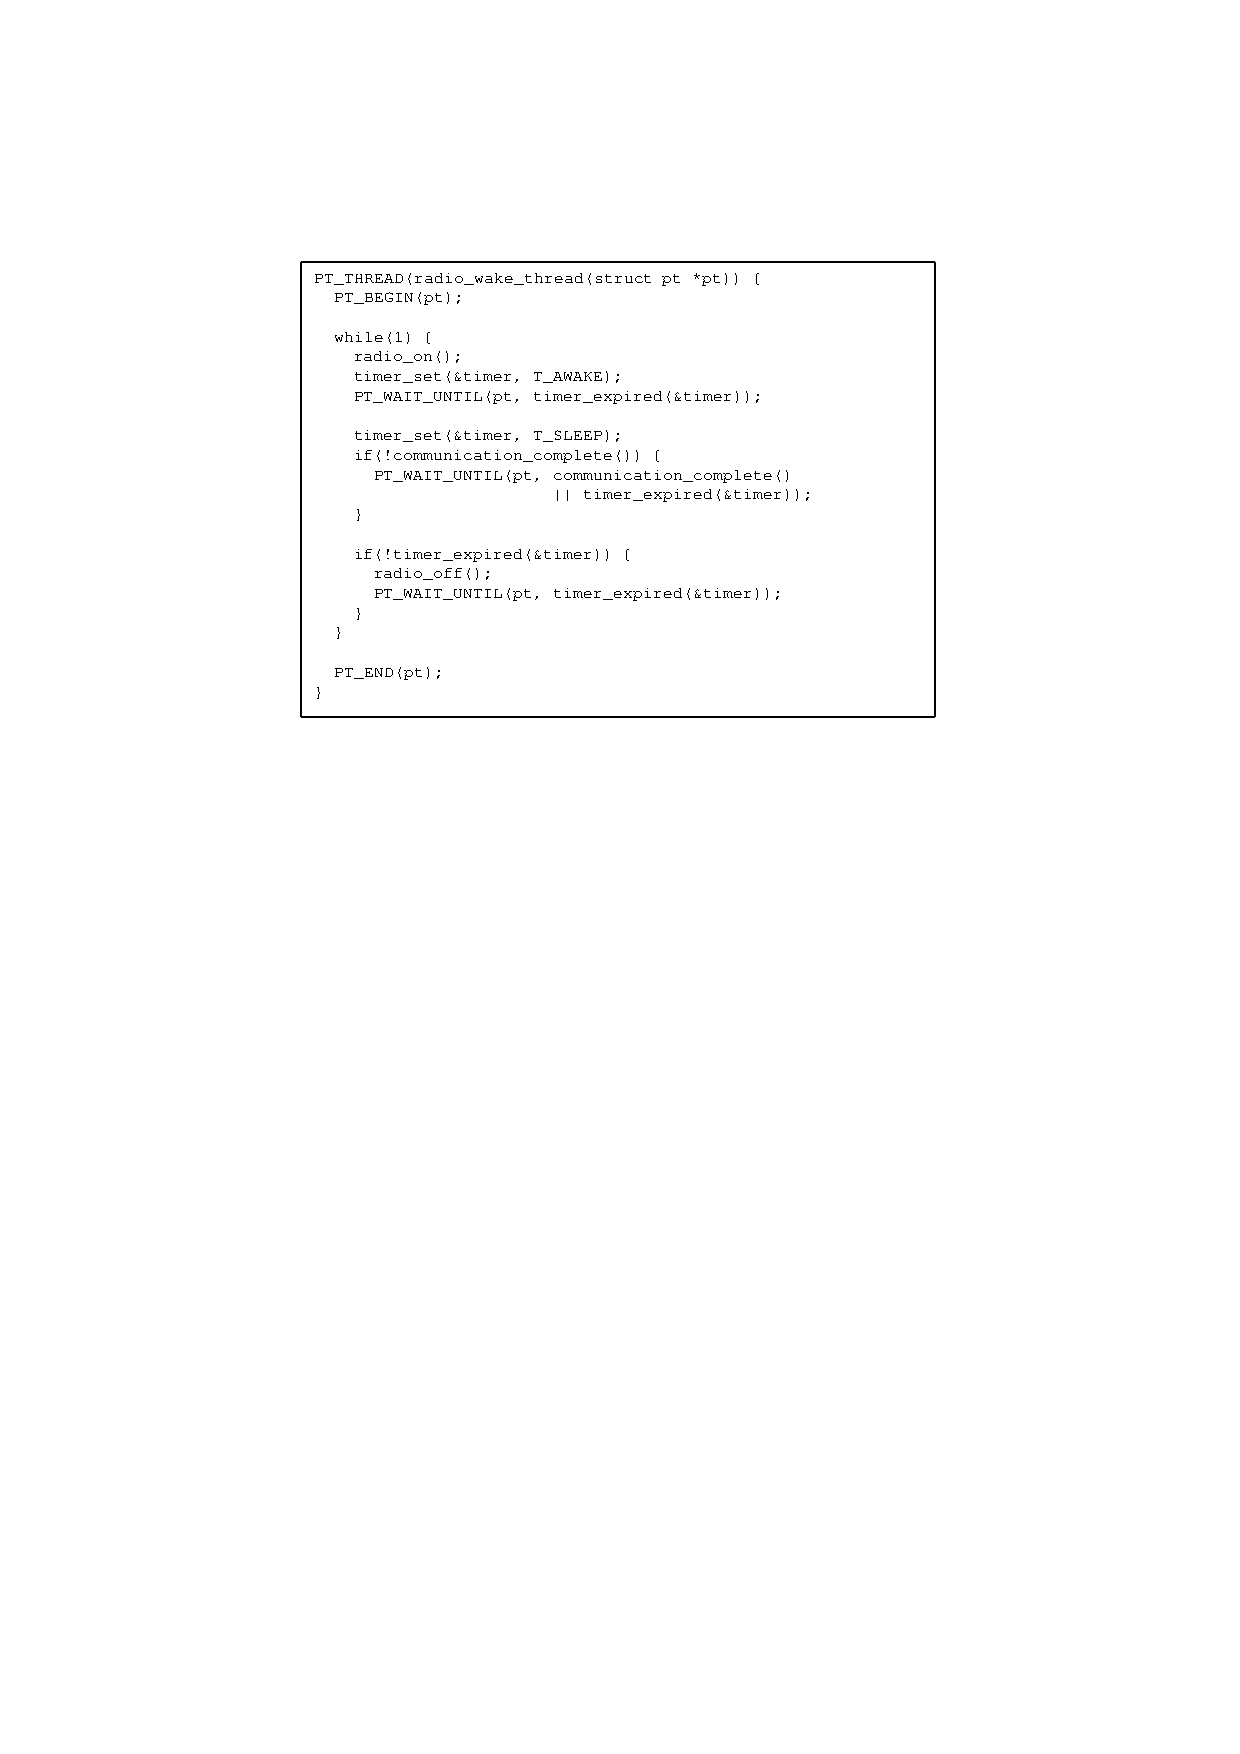
\includegraphics[width=0.9\textwidth]{dunkels-protothreads-example}
   \caption{Example code for a radio transmission program utilizing Protothreads. From \citep[p.7]{dunkels2005protothreads}. FIX: Check copyright!}
   \label{fig:ptexample}
\end{figure}

In figure \vref{fig:ptexample} a code example using Protothreads is shown, in which a radio is awaken at a set schedule to wait for check for transmissions. Protothreads uses a concept called \emph{conditional blocking} which can be explained in the following way: the execution can't leave the thread until a conditional blocking statement is reached (macros prefixed with `PT'). This can also be referred to as \emph{cooperative multitasking} as control can only leave a program when it voluntarily relinquish it.

As all Protothreads share the same stack and Contiki only needs to remember at which conditional to resume the thread, memory requirements can be as small as 2 bytes of RAM per thread. Furthermore, curiously enough, the `context-switching' mechanism can be wholly implemented using only the C switch control structure. This `quirk' of the C language was probably first discovered by Tom Duff\citep[p.10]{dunkels2005protothreads}\cite{wiki:duffs}.

%Programs written for an event-driven model typically have to be implemented as ex- plicit state machines. In contrast, with protothreads programs can be written in a se- quential fashion without having to design explicit state machines. To illustrate this, we return to the radio sleep cycle example from the previous section.

%\paragraph{Hardware support}
%From 8-bit to 32-bit Cortex M3. Requires bla bla ROM and RAM.

%Support for many 802.11.4 devices.


\subsection{IP networking}
UDP, TCP as well as ICMP over IPv4 and IPv6 are provided by the $\mu$IP stack, described in\cite{dunkels2003full}. The system is surprisingly robust given that its footprint amounts to only ~10 kB of ROM and a couple of hundred bytes of RAM: it fulfills all necessary host-to-host requirements stipulated in the relevant RFC documents\citep[p.4]{dunkels2003full} (e.g. flow and congestion control). The number of TCP connections and the size of the transmission / reception buffers are only limited by available RAM.

\begin{figure}
   \centering
   \begin{minipage}{.5\textwidth}
      \centering
      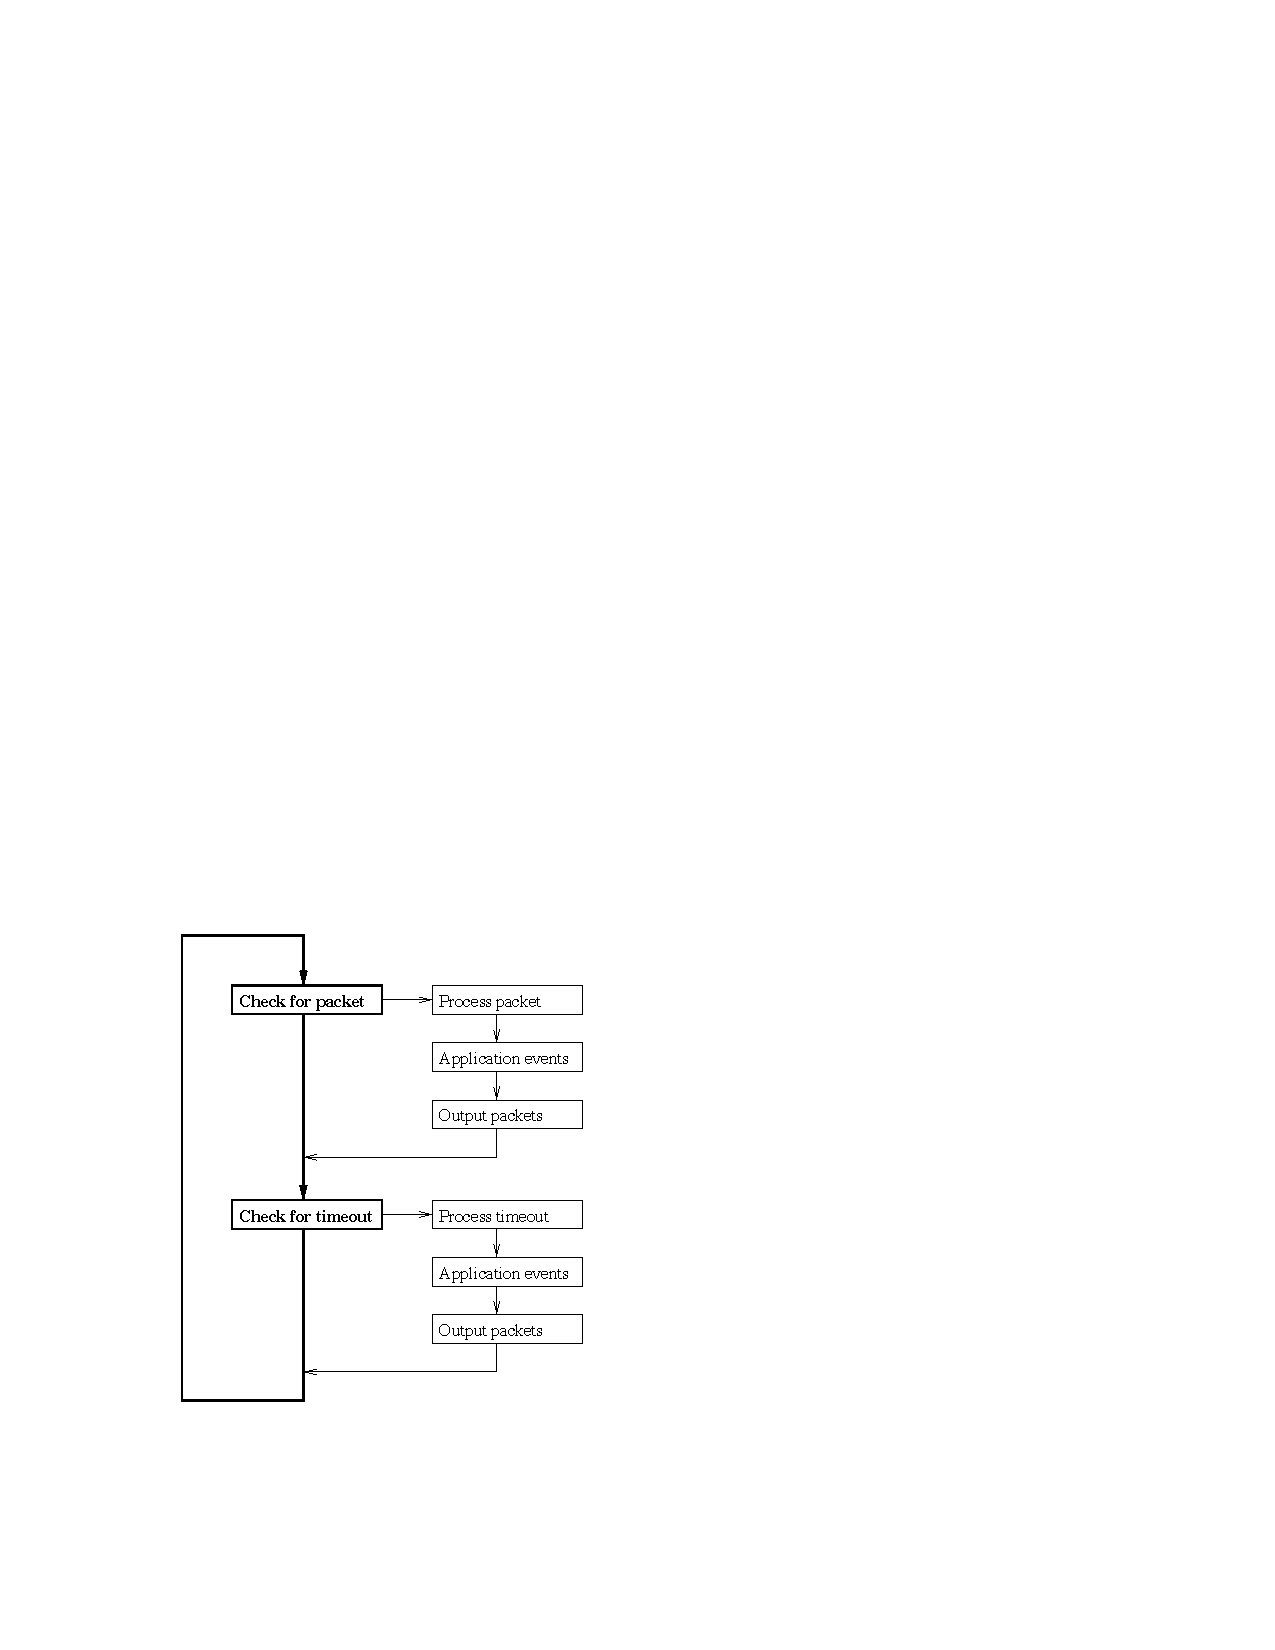
\includegraphics[width=.9\linewidth]{dunkels-uip-main_loop}
      \caption{$\mu$IP's main control loop. From \citep[p.6]{dunkels2003full}. FIX: Check copyright!}
      \label{fig:uip-ml}
   \end{minipage}%
   \begin{minipage}{.5\textwidth}
      \centering
      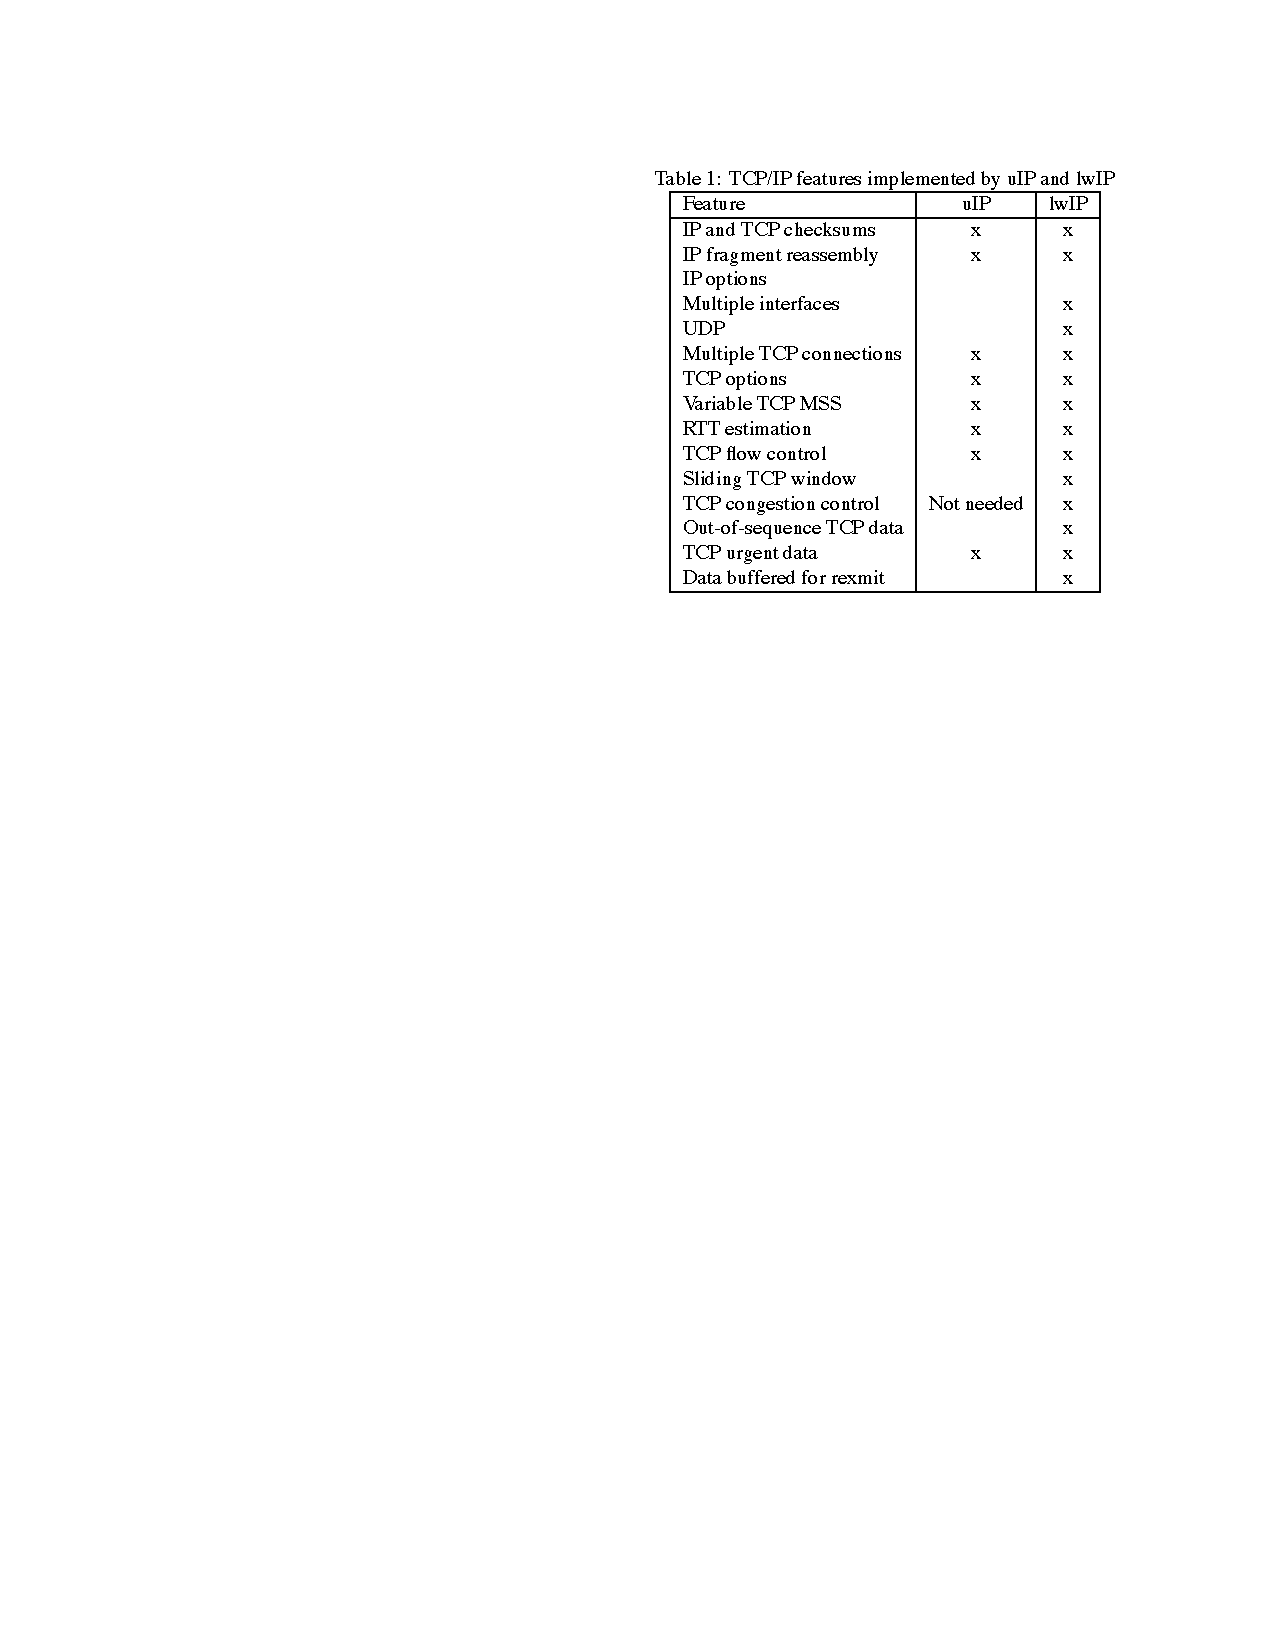
\includegraphics[width=.9\linewidth]{dunkels-uip-and-lwip}
      \caption{Features of $\mu$IP and the now no longer maintained lwIP. Since the table was published in \citep[p.4]{dunkels2003full} UDP has been added as well to $\mu$IP.}
      \label{fig:uip-features}
   \end{minipage}
\end{figure}

One important reason as to why $\mu$IP can achieve such a low memory footprint is that is liberates the OS from the complicated transmission of data between application and IP stack. Most of the requirements associated with this interface, as described in the RFC, are waived in \citep[p.4]{dunkels2003full}. This not only removes the need for a lot of software logic, but also allows a drastic simplification of transmission buffer management, something which its designer have used to the fullest extent: there is only enough buffer space for one packet at any time, including the need of transmissions as well as receptions. Figure \ref{fig:uip-ml} describes the main loop of $\mu$IP which explains its buffer management. The application that wish to transmit data copies it into $\mu$IP's buffer and then calls the transmission function with the appropriate addressing information. Upon reception, the procedure is the opposite. The stack figures out which application is interested in the arrived piece of data, then calls its handler, which in turn is programmed to react on the data and to produce a reply, which in turn is written to the very same buffer and so on.

Even though an IP packet can be well over a kilobyte in size (the MTU\footnote{Maximum Transmission Unit: The largest size of a packet that a network or a host can handle.} of IPv6 is 1280 bytes), the buffer can still be much smaller than this if used in conjunction with a MAC\footnote{Media Access Control} layer that has a small MTU (6lowPAN (using IEEE 802.15.4 in turn) is very popular for Contiki and has a MAC MTU of at most 102 bytes\citep[section 4]{rfc4944}). This will allow the incoming IP-packet fragments to be spoon-fed to the receiving application, negating the need for a large buffer for transmission purposes. Buffer size then becomes a problem of how large IP-packets one wants the applications to transmit.

\section{Security of the Internet Protocol}
\paragraph{Security on the Internet} was, and is, as of today an unresolved issue in my opinion. As its protocol, IP, was originally designed and developed in the open world of academic computer science, no security considerations were made. Instead, the three properties of information security (confidentiality, authenticity, integrity) \citep[section 8.1]{vasseur10interconnecting} were provided by physically protecting the network's hardware and the imposition of social norms among its users and operators. As the Internet grew, this and other weaknesses started to become problems. In 1995, the IETF\footnote{The Internet Engineering Task Force is the governing body of the development of Internet standards.} released a number of documents starting with RFC\footnote{RFC, or Request For Comment, is the collective name of the IETF's standards} 1883\cite{rfc1883} that defined IPv6, the planned successor of IPv4. Since security had become a concern at the time of its design, provisions for secure communication was included, and this part of the IPv6 standard was named IPsec\footnote{I should be noted that with RFC 6434\cite{rfc6434} in late 2011, the requirement that all IPv6-compliant hosts must feature IPsec functionality was dropped.}. This provided the network layer (the layer which IP operates on) and everything above it with secure communication.

% It was thought to address the question of security on the Internet in a conclusive manner, but as the Internet-wide deployment (or switch) to IPv6 still hasn't taken place, other solutions were invented and IPv6's approach of placing the security features in the network layer has been questioned.

However, adaption of IPv6 has been slow despite growing technical problems with the still incumbent IPv4. The resistance to upgrade is widely attributed to the fact that the cost and risk (software adaption, operator training, equipment replacement etc) of making the change in most networks outweighs the potential benefits. This equation will certainly change, if slowly, in the coming years. In the meantime, IPv6 has been found to be a great boon to new networks like Internet-connected smart phones, Internet-enabled set top TV-boxes and, naturally, the Internet of Things. In these cases it can be argued that the cost of adopting the legacy IPv4 is roughly the same as that of adopting IPv6, while enjoying benefits of the latter's simplicity, auto configuration features and more\footnote{See chapter 15.1 in \cite{vasseur10interconnecting} for a brief discussion about the benefits of IPv6 over IPv4 in the context of IoT.}.


\section{IPsec}

\paragraph{IPsec is a suite of protocols} that secures IP packets in an end-to-end fashion. Flows of packets, distinguished by properties such as source and target address, transport layer protocol, etc can be defined and different security policies applied. The system is not only limited to \emph{host-to-host} packet flows, but also allows a host to act as a gateway (termed \emph{security gateway} in the IPsec standard), enabling a secure link between two networks (\emph{network-to-network}) or a network to a host (\emph{network-to-host}). The suite can be implemented either directly in the IP stack of a host, but may also be located between the link layer and the network layer\citep[section 3.3]{rfc4301}, facilitating retrofits of existing stacks.

The motivation of the IPsec system is to deliver the security services confidentiality, authenticity and integrity in the OSI\footnote{Open Systems Interconnection is the so called ideal network model consisting of a seven layer protocol `stack'.}  stack's network layer, thus securing all data at this level (namely IP packets) and everything that it encapsulates (which is all protocols on higher levels in the stack e.g. TCP, UDP, application protocols). The system is designed in such a way that each compliant host features a set of databases which stores security information such as encryption keys and mechanisms that performs cryptographic operations on IP packets using that information. The hosts uses two extension headers (AH and EPS, as discussed in \nameref{sec:uiphdr}) to communicate security metadata between the hosts. More complex tasks like key negotiation is carried out by a so called key management protocol, one of which is IKEv2 (described in \prettyref{sec:ikebg}). Now, in this section I will introduce IPsec by describing the components that process the IP packets using information stored in the databases. Then, I will continue in \prettyref{sec:uiphdr} by describing the aforementioned extension headers which are used to pass the security meta data between the IPsec hosts.

%\paragraph{IPsec provides confidentiality, authen, ... } between these hosts or networks. It 


\begin{figure}[h!]
   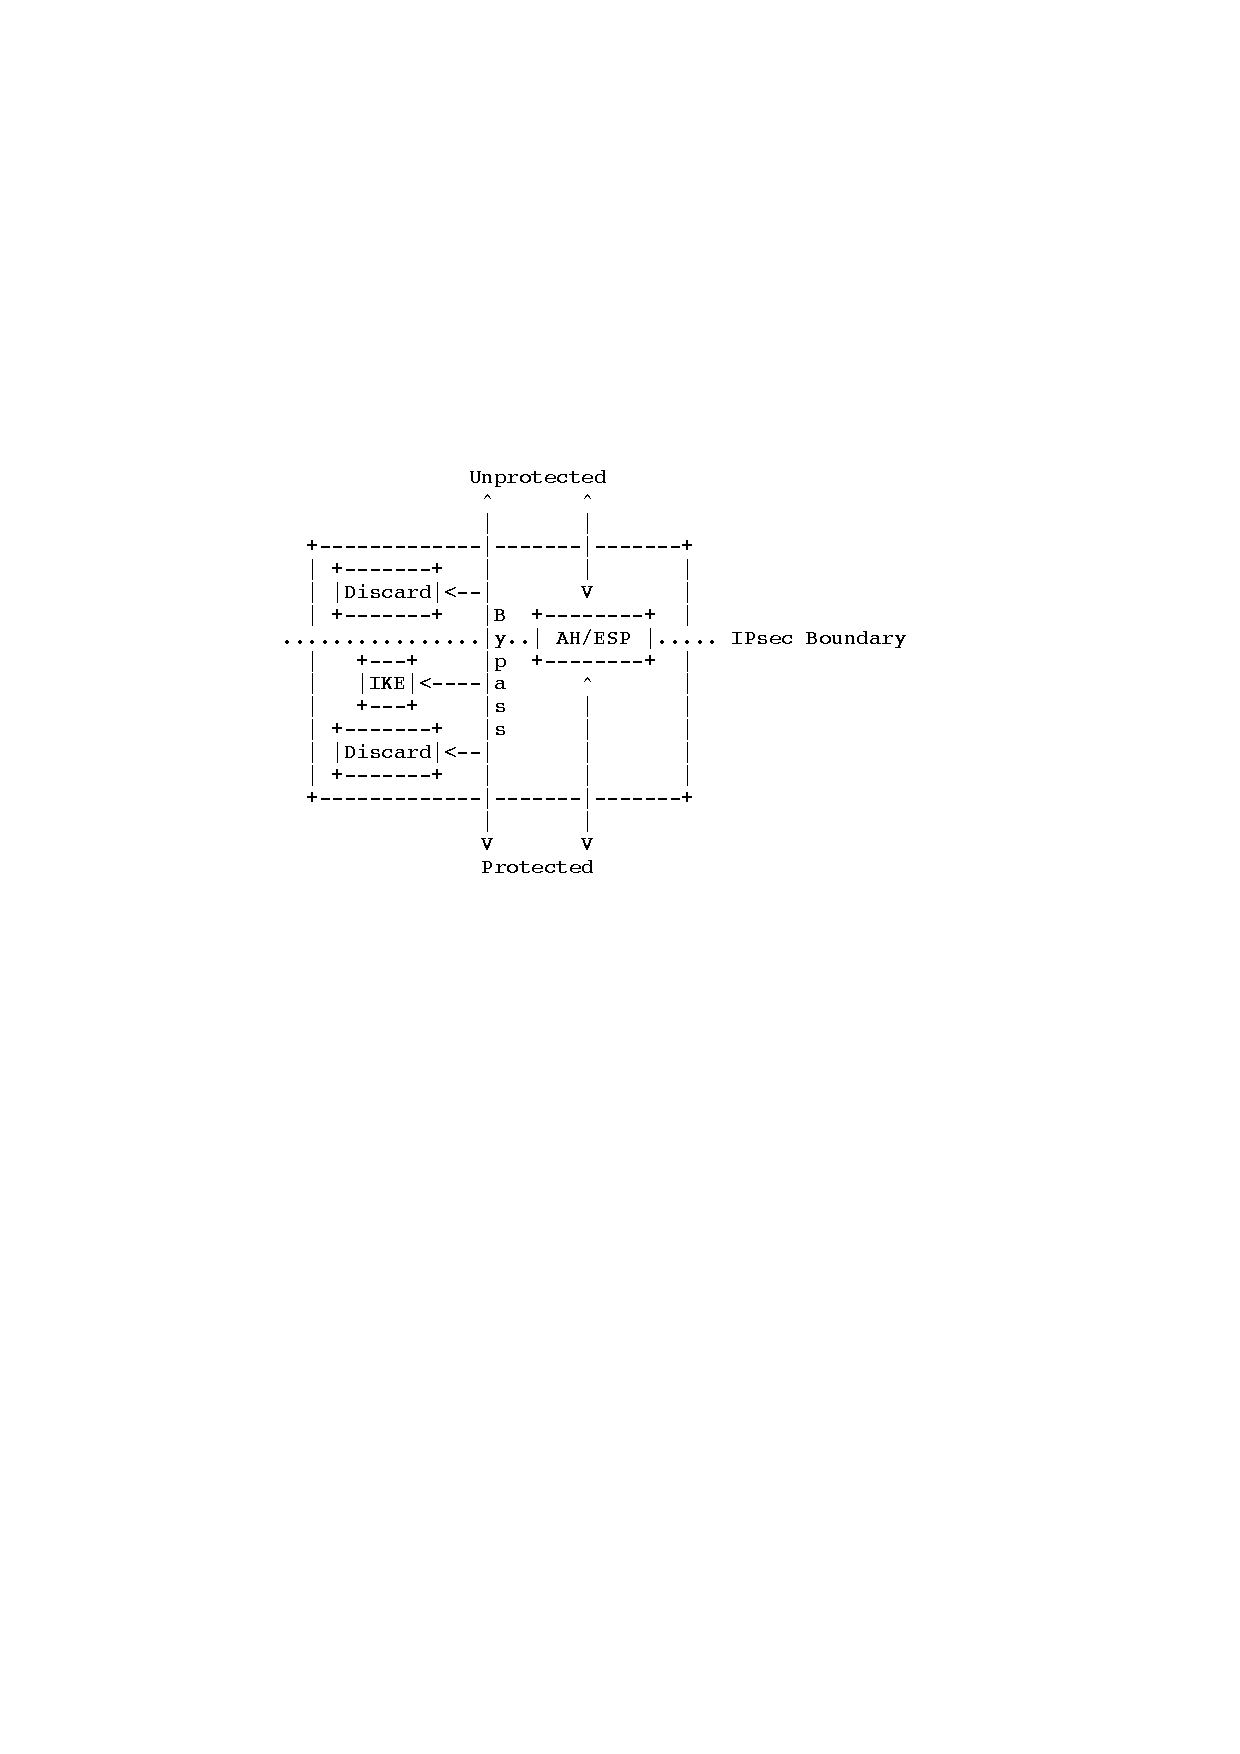
\includegraphics[width=0.9\textwidth]{ipsec-flow}
   \caption{IPsec processing of IP-packets. From \citep[p.8]{rfc4301}.}
   \label{fig:ipsec-flow}
\end{figure}

\paragraph{In the IPsec processing model} \label{ipsec_proc}
IP-packets are said to be passed from \emph{protected} to \emph{unprotected} network interfaces and vice versa. In the usual case, such as above, there are only one of each. The unprotected interface is always the interface connected to the insecure network, while the protected may be either connected to a secure network (the \emph{security gateway} configuration) or be attached to an operating system's IP stack. The flow of packets between the protected and unprotected interfaces are determined by policies set by the system administrator which are expressed in terms of network- and transport-layer primitives, i.e. IP addresses, port numbers and transport-layer protocols. The policy can cause a packet to be: thrown away (\emph{DISCARD}); forwarded over the IPsec boundary without any action taken (\emph{BYPASS}; removing or applying cryptographic protection of the packet (\emph{PROTECT}). The latter is performed in the module named \emph{AH/ESP} in \prettyref{fig:ipsec-flow} which handles the decoding and encoding of the AH and ESP IPv6 extension headers (as discussed in length in \prettyref{sec:uiphdr}).
   
\paragraph{IPsec affords protection for the traffic passed between networks as well as that between individual hosts.} In the former case, two IP networks are linked to each other by an IP-tunnel\footnote{An IP-tunnel allows communication between two IP-networks that don't have a routing path between each other. As the packets are transported by means of encapsulation (one IP-packets is transported in the payload field of another), other protocols can be `tunneled'  as well.} with an IPsec host at either end, acting as \emph{Security Gateways}. Packets that are routed to the other host's network are encapsulated in a security container (so called AH and ESP headers, which we will explain in \prettyref{sec:bgah} and \prettyref{sec:bgesp}) and dispatched to the Security Gateway at the other end of the tunnel. This allows secure communication between two networks and is useful when their hosts are not configured for IPsec. This mode of operation is referred to as \emph{tunnel mode} in the standards documents.

Although tunnel mode is by far the most popular usage of IPsec, this thesis will not implement it as it becomes less relevant in an IoT environment, for a variety of reasons described in \prettyref{cha:doi}. Instead, the research will focus on the so called transport mode\footnote{Transport mode as in transport layer mode} where no encapsulation takes place.

\paragraph{A central concept} of the IPsec model is the data structure named the \emph{Security Association} (SA). A Security Association defines a single simplex IP link and the security services it provides to the traffic that it carries. The services can be implemented by one of the two IPsec protocols: \emph{Authentication Header} (AH) and \emph{Encapsulating Security Payload} ESP. Bi-directional (duplex) traffic is enabled by creating a pair of SAs, one for each direction. As I will show, the SA is used by almost all IPsec components and we will return to it from time to time.

\paragraph{The policies and cryptographic secrets} used in IPsec processing are stored in three databases: the Security Association Database (\emph{SAD}); the Security Policy Database (\emph{SPD}) and its caches; the Peer Authorization Database (\emph{PAD}). The standard stresses the fact that the implementation of these databases should not be viewed as pre-requisites for a compliant IPsec implementation, but that such a system should exhibit the very same behavior as that of a system whose architecture was implemented in line with the standard's model. In the following paragraphs these databases will be used as constructs to explain the inner workings of IPsec, although, as the reader will learn in the \prettyref{cha:doi}, I have actually used these constructs in the final implementation as well. Finally, the system will be explained only in brief as the IPsec suite is simply too large for a thorough review in this thesis. The interested reader is advised to read the complete standard document\citep{rfc4301} starting at section 4.4 for an in-depth definition of the SAD, SPD and PAD.


\paragraph{The SPD} stores the policies that controls IPsec processing. It consists of an ordered list, where each entry is composed of a set of \emph{selectors}, \emph{PFP flags} and a \emph{processing action}. 

The \emph{selector} is a data structure that represents a traffic pattern between hosts or networks and serves to distinguish what traffic the policy in question is referring to. The fields are as follows: Local address; Remote address; Next Layer Protocol (e.g. TCP, UDP, ICMP); Local Port (This is dependent upon protocol type, e.g. in the case of an ICMP packet message type and code is listed instead.); Remote Port. Full specifications are found in \citep[Section 4.4.1.1]{rfc4301}.

PFP, or \emph{Populate From Packet} flags, are rules used in conjunction with the instantiation of an SA on the basis of the SPD entry. Instantiation in this context means that the newly created SA's selector (which has a similar purpose to a SPD entry's selector) is completed with information from that of the SPD entry's selector. However, for each of the selector's fields there is a corresponding PFP flag. If that flag is set, that field will be populated with information from the packet that triggered the instantiation. This process will be explained in detail further on as it's a central mechanism.

The \emph{processing actions} are the very same as described in \ref{ipsec_proc}: \emph{DISCARD}; \emph{BYPASS}; \emph{PROTECT}. The action \emph{PROTECT} differs from the the other actions in the sense that is also includes settings of how to protect the traffic, e.g. using a security gateway (tunneling), DSCP\footnote{Differentiated Services Code Point; QoS for IPv6} services, various SA settings used in instantiation.

\paragraph{The SPD's caches} can be divided into three different sections: SPD-O outbound traffic that is not to be protected; SPD-S for outbound traffic that is to be protected; SPD-I for all incoming traffic. The entries contains the same fields as the SPD, with the exception of the PFP (`Populate From Packet', as described above) field which is not present. From a functional point of view, each entry is an \emph{instantiation} of an SPD entry. That implies that each entry's selector is a subset of one of the SPD's entry's selectors. The IPsec processing mechanism creates such entries in response to encountering traffic that uses one of the SPD's entries. This is made because of two reasons: 

\begin{quotation}
1) Lookups in the SPD can be slow on large systems with many SPD entries. The SPD cache is faster\footnote{As to the question of why the SPD's cache allows a faster lookup, I have to direct the reader to RFC 4301. This speedup is hardly relevant to the thesis in question and thus the curious reader is encouraged to start reading at section 5, taking extra care to read the parts about de-correlation.}.
\end{quotation}

\begin{quotation}
2) a rule in the SPD can order traffic for a large address space to be protected. That address-space can contain many hosts, and each host can in turn demand different SAs for different traffic (e.g. different SAs for traffic over TCP and UDP). Thus, one realizes that each SA must explicitly define what traffic it carries. This is one of the purposes of the SPD-S cache. Each entry corresponds to an SA and its selector defines its traffic.
\end{quotation}

It's unfortunately hard to get a good overview of the SPD's caching system as the information is sprinkled over large parts of RFC 4301. I recommend the curious reader to begin reading at section 5, `IP traffic processing'\citep[Section 5]{rfc4301}.



% SPD-S outbound prot. traffic: Selectors and more goes here for instansiated SAs
% SPD-O outbound nonprot. traffic: fast lookups
% SPD-I inbound nonprot traffic: fast lookups

%There is nominally one cache per SPD.

% The IPsec implementation context determines how selectors are used. For example, a native host implementation typically makes use of a socket interface. When a new connection is established, the SPD can be consulted and an SA bound to the socket. Thus, traffic sent via that socket need not result in additional lookups to the SPD (SPD-O and SPD-S) cache. In contrast, a BITS, BITW, or security gateway implementation needs to look at each packet and perform an SPD-O/SPD-S cache lookup based on the selectors.

\paragraph{The SAD} stores the IPsec system's \emph{Security Associations} (SAs). The purpose of the database is to store the parameters of the system's SAs, but can be used to store other information as well. RFC 4301 outlines in section 4.4.2.1 fifteen required fields and because of space constraints, this section will only list the ones that I deem most important.

Security Parameter Index (SPI): Each SA is identified by a 32-bit value. This value is selected by the receiving end of an SA to be unique. This makes it possible for a system to uniquely associate inbound traffic with an SA using the SPI number as the key. Outbound traffic processing uses the SPI number to construct the IPsec headers.

Sequence Number Counter: Every IPsec system maintains a counter for each SA that is incremented by one for each packet that it carries. This information is used in IPsec packet processing and anti-replay protection (as will be explained below.)

Anti-Replay Window: A counter and a bit-map used for detecting packets that have been replayed by an attacker\label{mitm}\footnote{In a replay attack, a packet is intercepted by a man-in-the-middle with the purpose of delaying or repeating it. This can trick the targeted system into revealing secret information e.g. reusing the same keys in a stream cipher.}. The anti-reply protection is available for the AH as well as the ESP security protocols, but only when using automatic key management (more on this later).

Symmetric encryption information: Encryption algorithm and IPsec protocol type (AH or ESP) used by the SA along with necessary secrets (keys etc) and parameters.

SA Lifetime: A limit at which the SA should be terminated, expressed in either time or the number of bytes transported by the SA.

%each containing the parameters of , each consisting of the following substructures: a \emph{selector}, and an \emph{action}.


\paragraph{The PAD} (section 4.4.3) is controlled by the administrator and used by the security association management protocol along with the SPD to negotiate new SAs. The core purpose of the database is to store 1) the identification tokens of the peers that the system is allowed to communicate with and 2) the authentication mechanism, parameters and data of each aforementioned peer.


% stores the authentication requirements for 5. As SAs can be created both manually by an administrator as well as automatically by a Key Exchange service such as IKE, 

%Security policies are stored in in the \emph{Security Policy Database} (SPD). It consists of several entries, each consisting of the following fields: a \emph{selector} that defines a certain traffic flow; . The selector includes source address range, destination address) by means of \emph{}
% 
%  are said to be members of a communication session for which the same security policies are applied. Such sessions can be   that can be implemented directly in the IP stack of a host or in a router 

% \paragraph{IPsec's security model} differs from that of the one commonly used by security protocols operating in the higher layers e.g. TLS and SSH. Instead of using primitives such as user identity or tickets to create secure connections or make policies, IPsec  uses the concept know to IP such as hosts, networks and upper layer protocols such as TCP or UDP.  and .. primitives known to IP; ports, transport layer protocols, networks and host IP-addresses. 
% 
% host-to-host
% network-to-network
% SAD
% SPD

\section{Understanding the IP headers}
\label{sec:uiphdr}
Understanding IP headers are key to understanding IPsec. I will therefore quickly review the structure of the IPv6 headers before moving on to explain their relationship to IPsec. Below the readers finds a schematic of the IPv6 header, also called the IPv6 `fixed header' for reasons that soon are to be discussed.

\begin{figure}[here]
   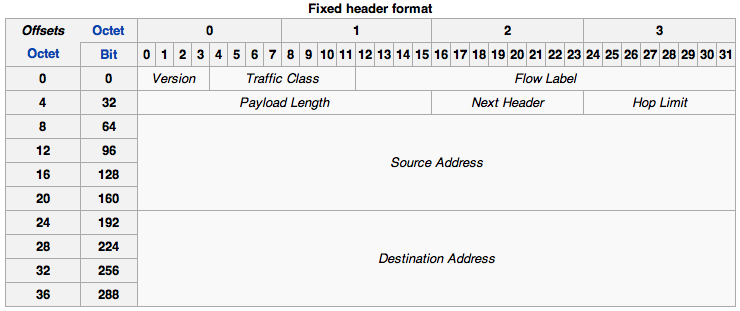
\includegraphics[width=0.9\textwidth]{wiki-ipv6-header}
   \caption{The IPv6 header. Figure from \cite{wiki:ipv6_packet}.}
   \label{fig:ipv6_packet}
\end{figure}

I assume that the reader is acquainted with the general principles of IP networking, the discussion of the above header fields will be brief. \emph{Version} is always six; \emph{Traffic Class} (reminiscent of the IPv4 \emph{TOS} field) and \emph{Flow Label} are for flow and congestion control, which are of no concern to us; \emph{Payload Length} is the length of the payload field, including any so called `extension header' (more on this soon); \emph{Next Header} specifies the packet's transport layer protocol, or the first extension header's type if one is present; \emph{Hop Limit} is equivalent to IPv4's Time-To-Live field which is decremented by each router along its path, ultimately to be discarded when it reaches zero.

IPv4 placed all of its settings into one big header, many settings which as of today are rarely used, and the possibility of extending it with new features are severely limited. The designers of IPv6 solved this problem by keeping the fixed header (figure \ref{fig:ipv6_packet}) small and allowing it to be extended by a mechanism called \emph{extension headers}. The extension headers contain any optional information, information which can be intended for the packet's destination host and/or intermediate routers along its path. Although the information is usually supplied by the source host, some headers (such as \emph{Fragment}) can be altered and/or added by routers.

\begin{figure}[here]
   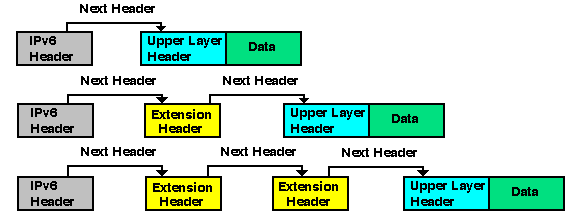
\includegraphics[width=0.9\textwidth]{ipv6-nextheader}
   \caption{Illustration of IPv6's next header scheme. FIX! Not received permission! Source:http://www.zytrax.com/tech/protocols/ipv6.html}
   \label{fig:ipv6_nextheader}
\end{figure}

\begin{figure}[here]
   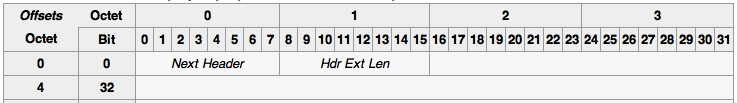
\includegraphics[width=0.9\textwidth]{wiki-ipv6-nextheader}
   \caption{The generic mandatory part of an `extension header'. Figure from \cite{wiki:ipv6_packet}.}
   \label{fig:wiki-ipv6-nextheader}
\end{figure}

The extension header scheme is basically a linked list (figure \ref{fig:wiki-ipv6-nextheader}). The field \emph{Next Header} denotes the type of extension header to come or, if this is the last extension header, the packet's type of transport layer; \emph{Hdr Ext Len} is the length of this extension header in multiples of eight octets, not including the first eight octets. The rest of the next header contains data that is specific to each next header type.

\begin{figure}[h!]
   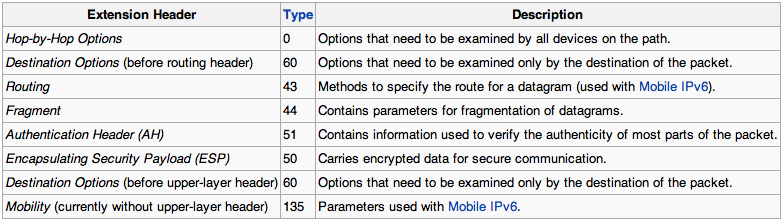
\includegraphics[width=0.9\textwidth]{wiki-ipv6-listofextensionheaders}
   \caption{This list covers a number of common extensions headers `next header'. List from \cite{wiki:ipv6_packet}.}
   \label{fig:wiki-ipv6-listofextensionheaders}
\end{figure}


\section{The AH protocol in IPv6}
\label{sec:bgah}

\begin{figure}[h!]
   % 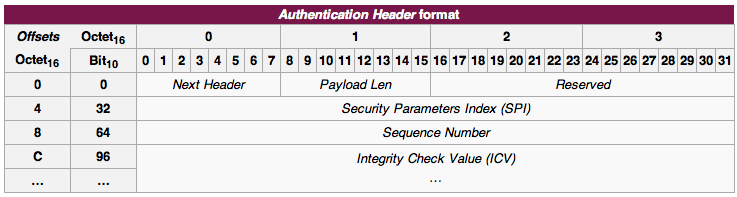
\includegraphics[width=0.9\textwidth]{wiki-ipsec-ah}
   % \caption{The AH extension header. From \cite{wiki:ah_header}.}
   % \label{fig:wiki-ipsec-ah}

   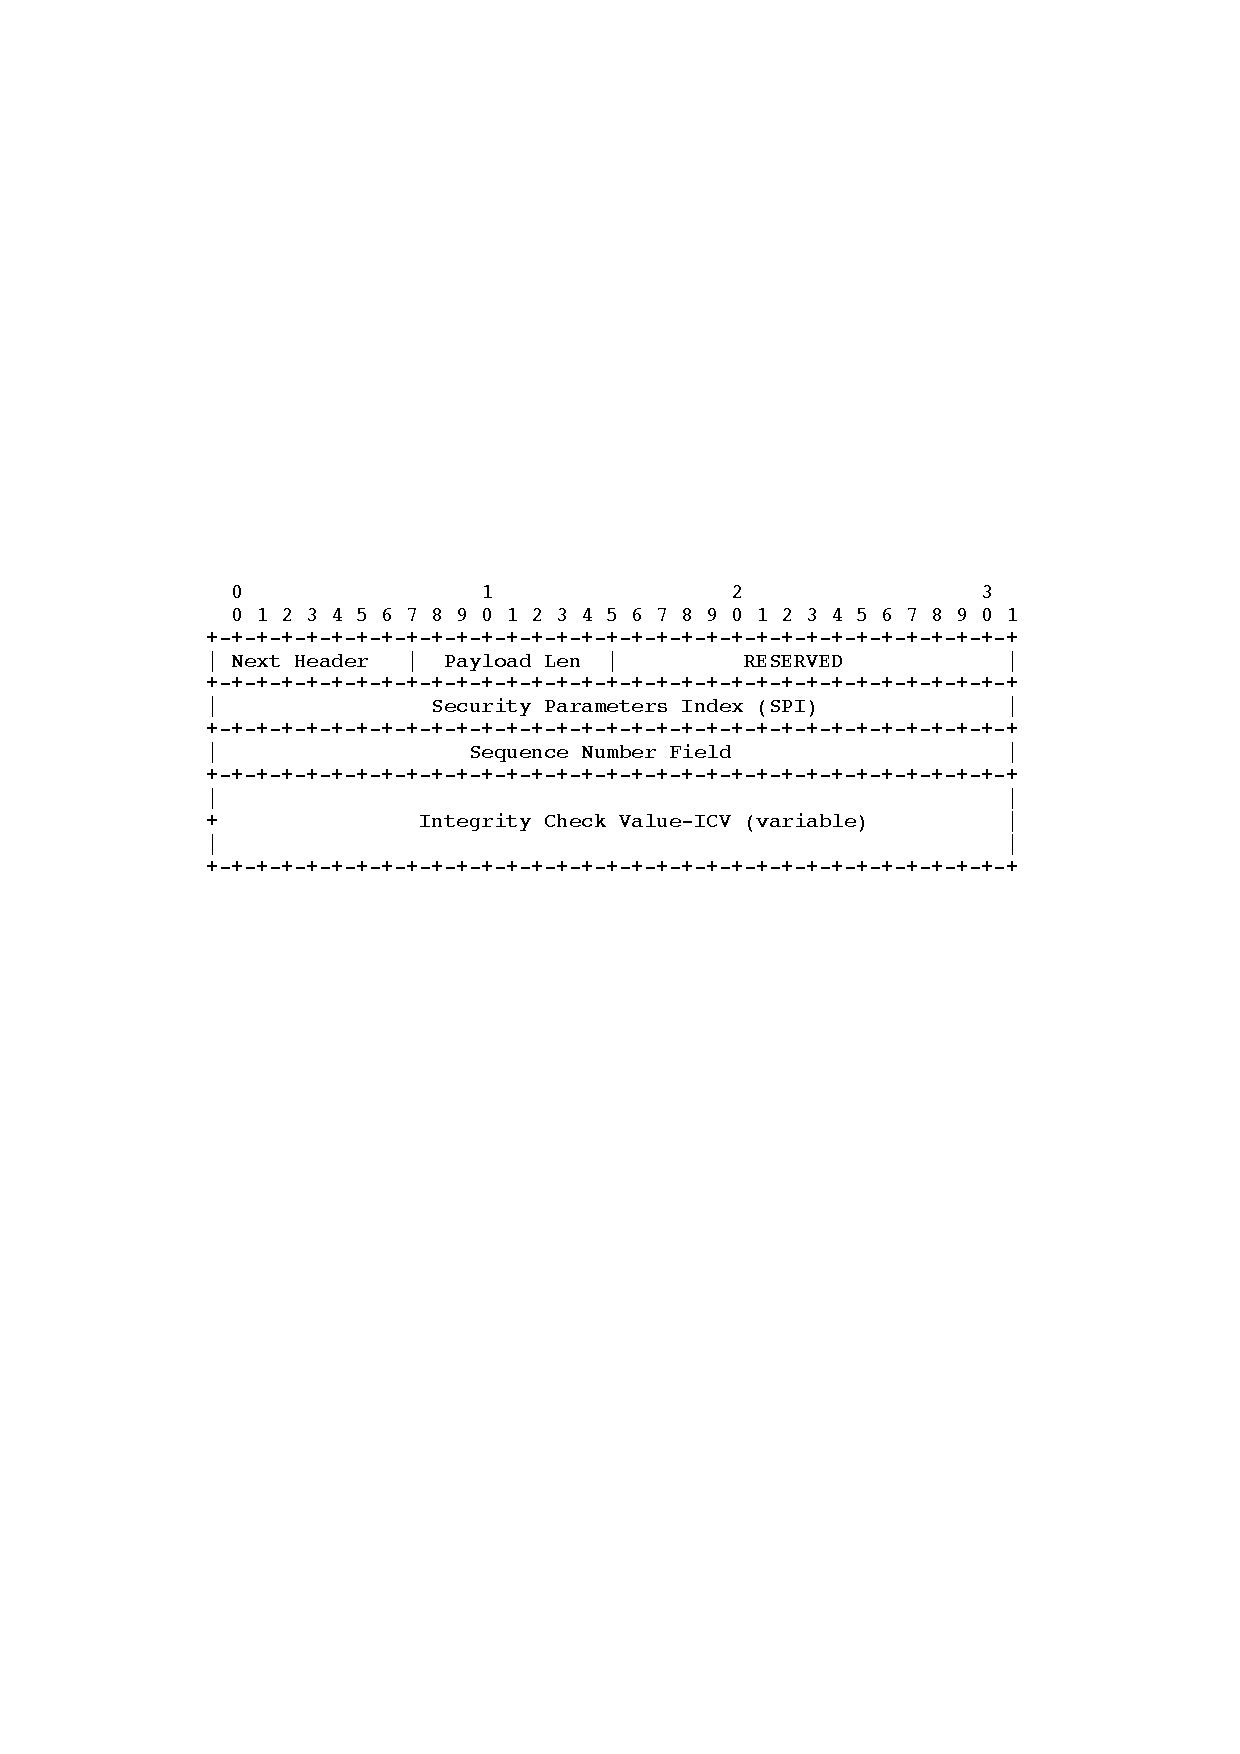
\includegraphics[width=0.9\textwidth]{ah_nextheader}
   \caption{The AH extension header. From \cite{rfc4302}.}
   \label{fig:wiki-ipsec-ah}

\end{figure}

The AH protocol's header (\emph{Authentication Header}) described in RFC 4302\cite{rfc4302} guarantees the \emph{data integrity} and the \emph{data authentication} (origin) of the IP packet which it is applied to. This is achieved by applying a \emph{Message Authentication Code} (MAC) to the packet's content and to the header's immutable fields using a key privy to the two parties.

\begin{figure}[h!]
   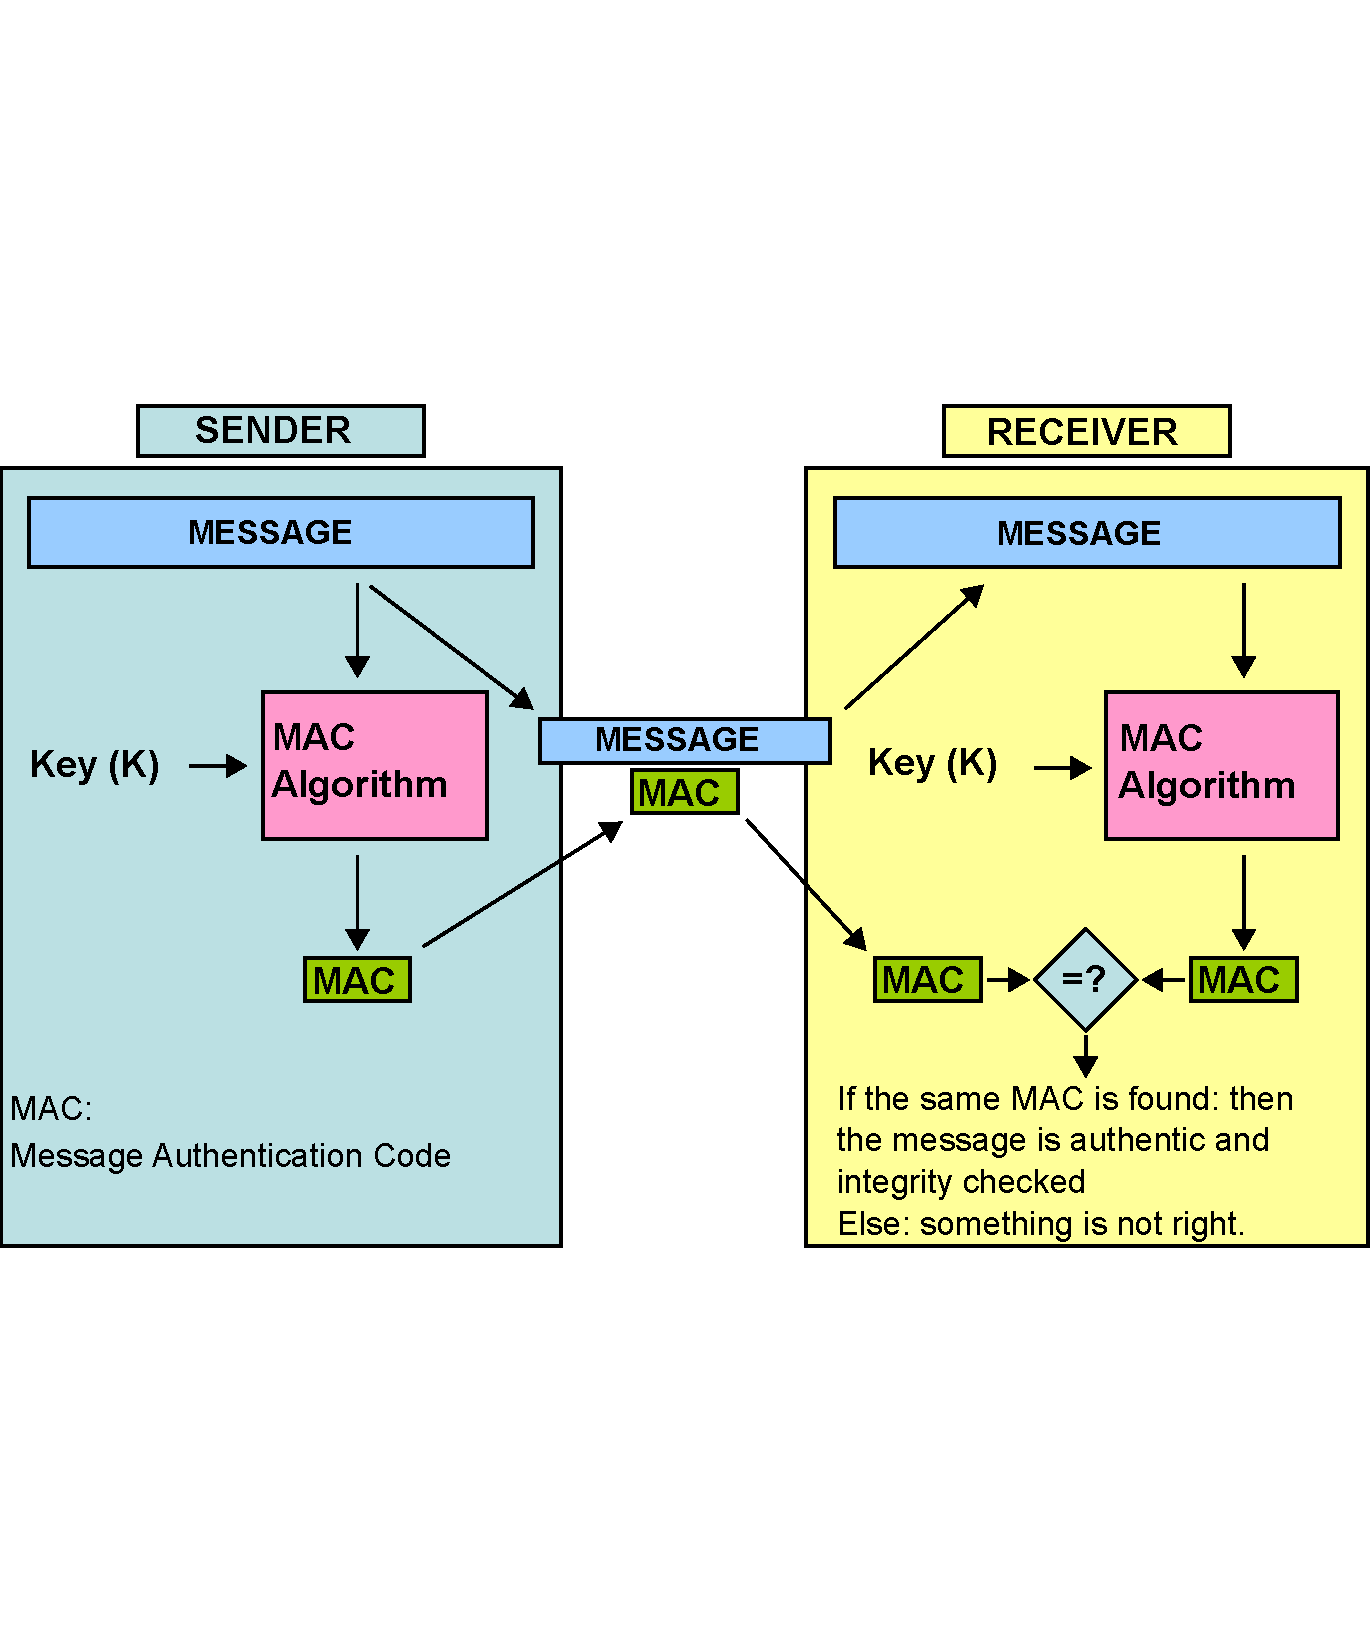
\includegraphics[width=0.9\textwidth, trim=0 205 0 210]{wiki-mac}
   \caption{Message Authentication Code. From \cite{wiki:mac}.}
   \label{fig:wiki-mac}
\end{figure}

Figure \ref{fig:wiki-mac} describes the principles of a MAC algorithm: The message, composed of the packet's payload and its immutable fields, are combined and digested\footnote{A synonym of \emph{digested} is \emph{hashed}.} along with a key. This produces a \emph{MAC} string (also referred to as a \emph{digest} or \emph{hash} string) which is attached along with the message. IPsec refers to this value as the \emph{ICV}.

Upon arrival the receiver performs the same calculations and compares the resulting \emph{MAC} with that included in the packet. This scheme will, if correctly implemented and algorithms chosen with care, make it computational infeasible\footnote{A security attack is said to be `Computationally Infeasible' if the required cost of performing the necessary cryptographic computations are outside the reach of even very large organizations.} for an attacker to alter the message without knowledge of the key. As a side benefit, the packet is also protected against accidental corruption such as transmission errors.

The parameters of the process (such as key, key length and type of MAC algorithm) are SA-specific and are stored in its data structure.




\section{The ESP protocol in IPv6}
\label{sec:bgesp}

\begin{figure}[h!]
   % 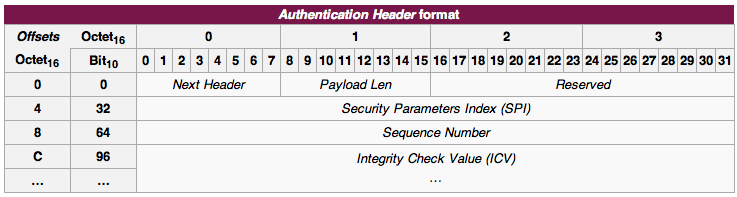
\includegraphics[width=0.9\textwidth]{wiki-ipsec-ah}
   % \caption{The AH extension header. From \cite{wiki:ah_header}.}
   % \label{fig:wiki-ipsec-ah}

   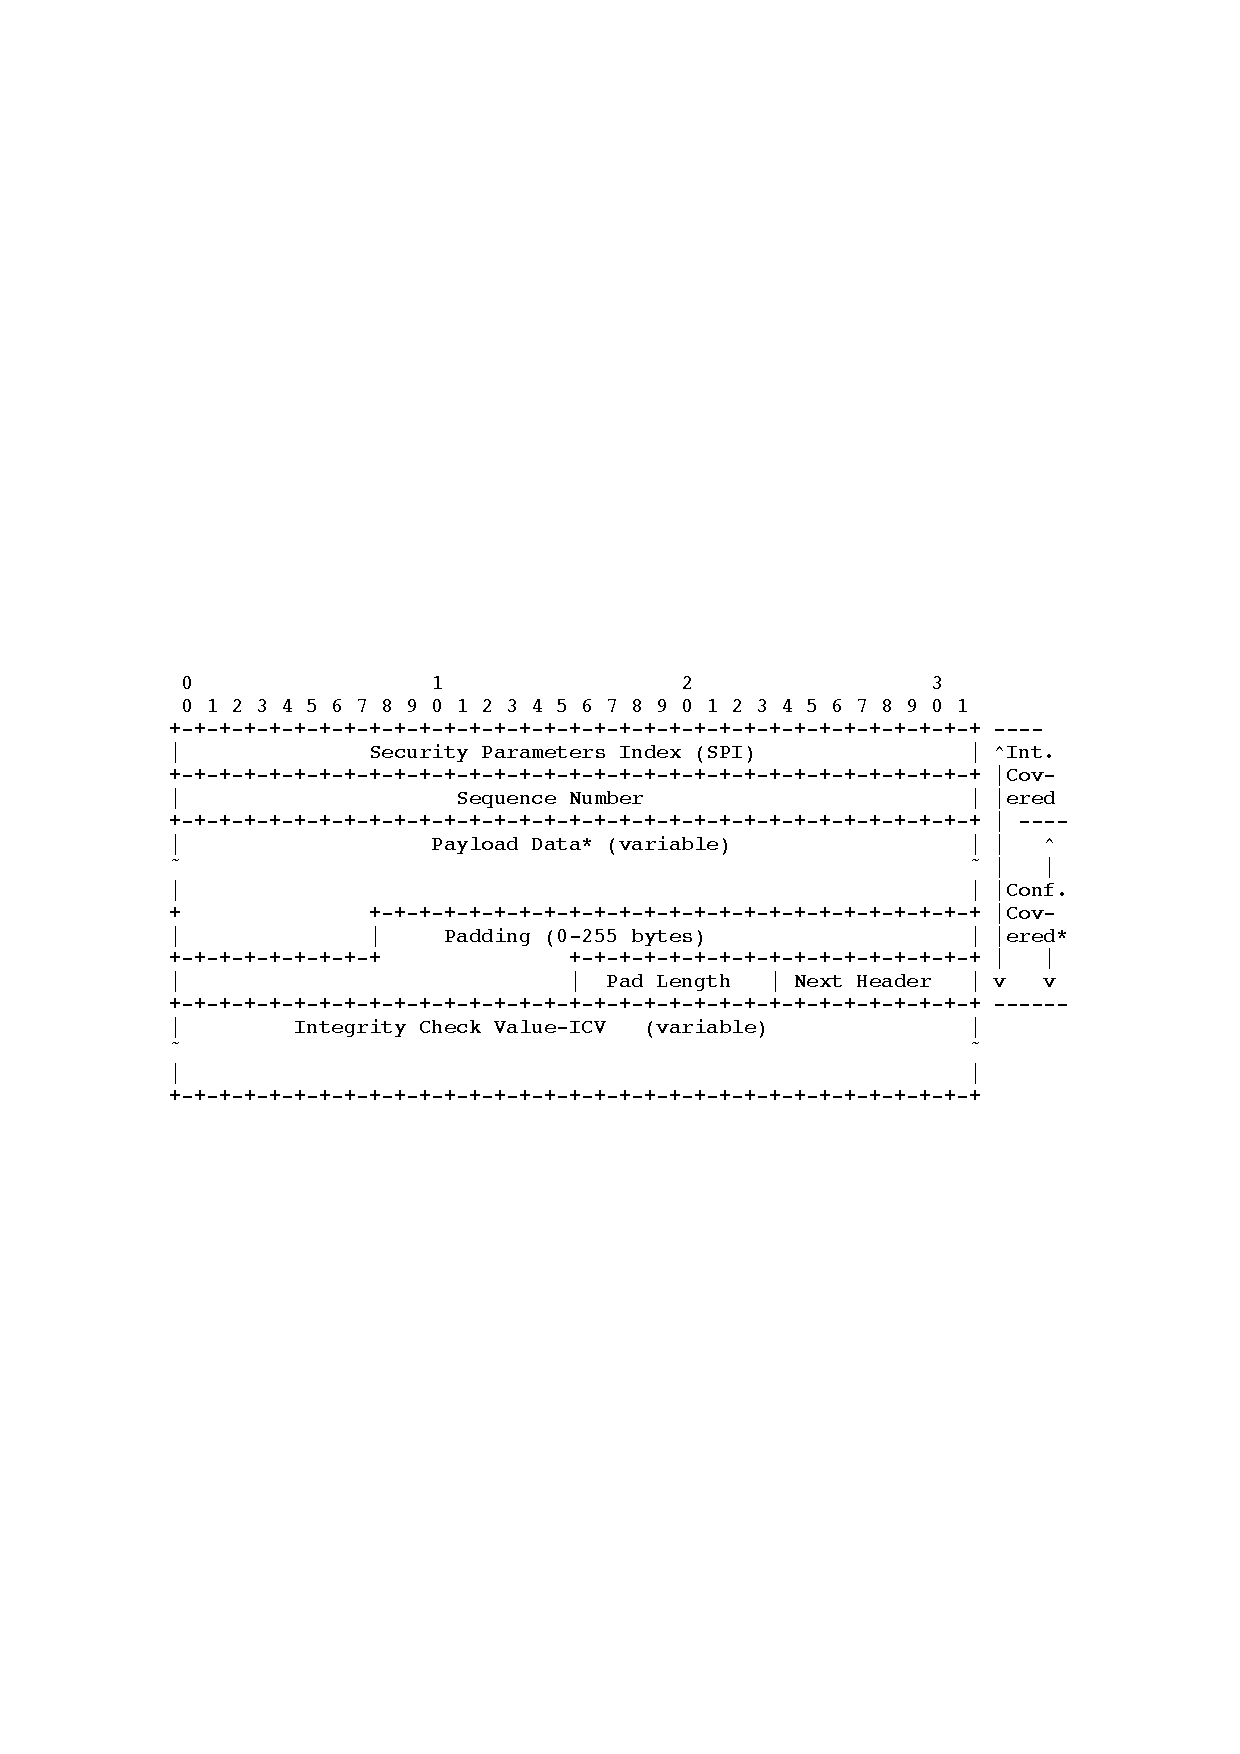
\includegraphics[width=0.9\textwidth]{esp_nextheader}
   \caption{The ESP IPv6 extension header. From \cite{rfc4303}.}
   \label{fig:wiki-ipsec-esp}
\end{figure}

The ESP (Encapsulating Security Payload) protocol described in RFC 4303\cite{rfc4303}, provides \emph{confidentiality} and limited \emph{traffic flow confidentiality} in addition to AH's \emph{data integrity} and \emph{data authentication}. The term \emph{Encapsulating} is derived from the fact that the protocol is designed to encase everything that follows it in the packet (extension headers as well as payload). This practice is of benefit in itself, but rather it facilitates the implementation of confidentiality protection. For example, there are many popular algorithms which belongs to the block cipher family e.g. AES-CBC. Such algorithms only operates upon fixed sizes of data and therefore needs to pad\footnote{To `pad' data is to prepend or append white space characters (in the case of text documents) or null bytes to a string in order to increase it to a predetermined length.} the IP packet's payload to a multiple of the block length.

The fact that confidentiality protection is optional makes ESP services identical to that of AH's, but only under certain circumstances. In \prettyref{cha:doi} it will be shown how this fact can be exploited.


% \cite{wiki:ipv6_packet}
% 
%  architecture has always been open
% * Protects everything from the network level and up (Model)
% * Symmetric encryption
% * Security associations
% 

\label{sec:ikebg}
\section{Automatic key management (IKEv2)}%{Automatic negotiation of SAs (IKEv2)}
We have now explained the essentials of IPsec: the databases and their relations to each other and how they govern the flow of packets in the IPsec stack. This functionality is all that is required for an interoperable IPsec implementation. However, this requires all SAs to be set by the administrators of the systems in question. I.e. if two such hosts wants to communicate by IPsec the administrators must agree upon, and manually create, the SAs along with their encryption keys and associated settings. Naturally, we would like to automate this in order to lessen the human's workload. This is the purpose of an IPsec Key Management Protocol. At of the time of this document's writing, there are several protocols: IKE (defined in RFC 2407 - 2409)\cite{rfc2407}\cite{rfc2408}\cite{rfc2409}; IKEv2 (RFC 5996)\cite{rfc5996}; KINK (RFC 4330)\cite{rfc4330} and IPSECKEY (RFC 4025)\cite{rfc4025}. What they all have in common is that they solve the problem of automated key management, albeit in different ways, and that they all interface with IPsec through its databases.

However, this thesis will henceforth only discuss IKEv2 as it's the de-facto standard and, more importantly, the original target of study for this work. IKEv2 is the successor to IKE that was widely regarded to be a standard that suffered from unnecessarily complicated and vague standards documents. This issues were addressed in IKEv2 and resulted in, most importantly: better interoperability among implementations; faster keying handshake; implementations with less complex codebase.

\subsection{Overview}
As previously stated, IKEv2 is a component that is wholly external to the parts that we have covered so far (IPsec packet processing, SPD, SAD etc). The former are usually, in a general purpose operating system, implemented in the kernel\footnote{Linux's current IPsec implementation follows this model, and I believe that Microsoft's equivalent for Windows does so as well.} while the latter is written as service running in user space. This is the preferred method on an IPsec host as IPsec's packet processing mechanism needs to be implemented in conjunction with the OS' network stack (referred to as `bump-in-the-stack' or `native' in RFC 4301\citep[p.10-11]{rfc4301}) while IKEv2 is shaped into a user-space service. Naturally, we want as much code as possible to run in user space as it facilitates development and allows better integration with the rest of the operating system.

\subsection{Negotiating SAs}
SAs are created when they are required; i.e. when an IP packet is about to leave the host or gateway towards a destination which, according to the policy in the SPD, requires IPsec protection of some sort. Such a packet can be either dropped\footnote{Remember that all parties in an IP-network must tolerate that IP packets are lost on occasion.} or stored for later transmission, depending on what suits the implementation best. Now, the IKEv2 service is ordered to establish suitable SAs (according to the security requirements entered in the SPD) with the remote peer in question. All traffic of the same pattern as that of the `triggering' packet will not be allowed to leave the peer until these SAs are established and entered into the SAD.

IKEv2 communicates with other IKEv2 capable hosts by means of UDP datagrams on port 500. As the purpose of the communication is to negotiate new SAs, the communication can not be protected by any IPsec SAs. Therefore, a correctly configured IPsec host must allow non-protected traffic on this UDP port. In this section I will explain how IKEv2 itself creates a secure communication channel for its datagrams.

I begin by quoting the standard; `All IKE [IKEv2] communications consist of pairs of messages: a request and a response. The pair is called an `exchange', and is sometimes called a `request/response pair'.'\citep[p.5]{rfc5996}. Every such request requires a response, and if none is received the sender of the request will re-transmit it until a response is received or a timeout occurs. 

The first exchange between two peers (hosts or gateways) that wish to negotiate cryptographic information for a secure communication channel (an SA, that is) is called the IKE\_SA\_INIT exchange. This will execute the so called Diffe-Hellman key exchange where a shared secret is formed between the peers without divulging it to eavesdroppers. The next exchange is the IKE\_AUTH exchange in which the peers authenticates themselves, thus preventing a man-in-the-middle-attack\footnote{Please see \ref{mitm}}. A secure connection is now established and the associated parameters are stored in a SA called the \emph{IKE SA}.

The IKE SA is only used by the IKEv2 service. Its sole purpose is to establish a secure channel by which the IKEv2 peers can create and destroy \emph{Child SAs}. Such a child SA pair (one for each direction) is now created with cryptographic material derived from the IKE SA (hence the term `child') in such a way that perfect forward secrecy\footnote{Keys derived from other, older keys, are said to be derived with PFS if it's performed in such a way that the disclosure of the older keys doesn't threaten the security of the new keys} is upheld. That pair is inserted into the SAD, thus completing the task.

The IKE SA is retained for future tasks such as re-keying, destruction or creation of more child SAs.


%This begins with the following exchange of data, as described in IKEv2 standards document, RFC 5996\citep[p.5]{rfc5996}:  


% \begin{quotation}
% All IKE communications consist of pairs of messages: a request and a response. The pair is called an `exchange', and is sometimes called a `request/response pair'. The first exchange of messages establishing an IKE SA are called the IKE\_SA\_INIT and IKE\_AUTH exchanges; subsequent IKE exchanges are called the CREATE\_CHILD\_SA or INFORMATIONAL exchanges. In the common case, there is a single IKE\_SA\_INIT exchange and a single IKE\_AUTH exchange (a total of four messages) to establish the IKE SA and the first Child SA. In exceptional cases, there may be more than one of each of these exchanges. In all cases, before any other exchange all IKE\_SA\_INIT exchanges MUST complete type, then all IKE\_AUTH exchanges MUST complete, and following that, any number of CREATE\_CHILD\_SA and INFORMATIONAL exchanges may occur in any order. In some scenarios, only a single Child SA is needed between the IPsec endpoints, and therefore there would be no additional exchanges. Subsequent exchanges MAY be used to establish additional Child SAs between the same authenticated pair of endpoints and to perform housekeeping functions.
% \end{quotation}

% The `IKE SA' referred to in the above text is an type of SA that is only for IKE communication. It is not used by the IPsec processing system, but only by the IKE service to secure its communication with other hosts. The creation of the `Child SA' is the final goal of the IKE connection - an SA to be used by the IPsec system to protect some part of the host's traffic. Its name can be derived from the fact that its cryptographic material is based upon that of the IKE SA's i.e. it can be said to be a descendent. On the next page (no. 6), the standard continues by providing more details about the SA negotiation:

% \begin{quotation}
% The first exchange of an IKE session, IKE\_SA\_INIT, negotiates security parameters for the IKE SA, sends nonces, and sends Diffie- Hellman values. The second exchange, IKE\_AUTH, transmits identities, proves knowledge of the secrets corresponding to the two identities, and sets up an SA for the first (and often only) AH or ESP Child SA (unless there is failure setting up the AH or ESP Child SA, in which case the IKE SA is still established without the Child SA). The types of subsequent exchanges are CREATE\_CHILD\_SA (which creates a Child SA) and INFORMATIONAL (which deletes an SA, reports error conditions, or does other housekeeping). Every request requires a response. An INFORMATIONAL request with no payloads (other than the empty Encrypted payload required by the syntax) is commonly used as a check for liveness. These subsequent exchanges cannot be used until the initial exchanges have completed.
% \end{quotation}
% 
% As UDP is an unreliable transport layer, IKEv2 includes a mechanism for retransmission:
% 
% \begin{quotation}
% An IKE message flow always consists of a request followed by a response. It is the responsibility of the requester to ensure reliability. If the response is not received within a timeout interval, the requester needs to retransmit the request (or abandon the connection).
% \end{quotation}
% 
% After the handshake is complete (i.e. the creation of the SA for the IPsec traffic), the IKE SA is retained for future use as this will negate the need to re-create it whenever child SAs shared with that particular host need to be created or destroyed.


%FSM diagram of a handshake??


% \subsection{Interfaces}
% (PICTURE) IPsec processing, SPD, SAD, PAD <-> IKEv2
% 
% As stated earlier, IKEv2 communicates with IPsec by manipulating its databases. However, what has not been mentioned is that the IPsec processing system can signal IKEv2 as well. One such case is when the need for a new SA arises. Consider the following scenario:
% 
% \begin{quotation}
% An application on the host sends data destined for another host. When the resulting packet is received by the IPsec processing mechanism it tries to determine wether or not the packet is to be protected by trying to match its destination address with the selectors found in the SPD and its caches. If found in SPD and req. prot. invoke IKE.
% 
%\end{quotation}

%The same procedure occurs upon SA expiration: expiration of an SA in the SAD causes IPsec to signal IKEv2 that it needs to negotiate a new one.


% \subsection{Putting it all together}
% Final review of IPsec processing mechanism

% SKRIV-ANTECKNINGAR
% 0715: Måste säga något om tunnlar. Vart lägger jag det?


% * Handshakes for IPsec
% * Establishing security associations
% * Asymmetric encryption



\chapter{Design and Implementation}
\label{cha:doi}

% Varför break:ar vi med standarden i Contiki? Varför är det fortfarande en implementation då?
Implementing Internet standards in Contiki is often a challenging task. The standards are written with the presumption of hosts with vastly more capable hardware, which requires the engineer to simplify parts of the standard, make generalizations, and omit other parts altogether. This might be difficult as it requires good knowledge of the standard in question as well as the behavior of other implementations. The synthesis of this knowledge allows her to save hardware resources by making shortcuts in her implementation, shortcuts which might very well violate the standard document, but still exhibit a behavior which allows communication with the rest of the Internet. This a good example of the very practical, experimental, approach that is typical of Contiki's development culture.

At this point I would like to remind the reader that most implementations of Internet Services are not standards compliant in one aspect or another, but may still be \emph{interoperable} with other implementations. This is especially true of more complex standards which describe many features. IPsec, for example, also describes APIs solely targeted towards the operating system's applications. These are surely neither applicable, nor necessary, in the context of IoT hosts. In this regard, violation of the standard documents is warranted as it will not hamper interoperability.

% The above statement may be confusing at this time; wasn't this thesis supposed to describe a complete implementation of IPsec and IKEv2? 
% While reading the following, the reader should keep in mind that most implementations of Internet Standards, are in factThe reader is advised to keep in mind that in the world of general purpose computing, there 

% How about illustrating the above with a quote from A's uIP-paper concerning RFC-compliance?

\section{Development process}
The original goal of this thesis was to develop a working IKEv2 implementation that would operate with an existing IPsec implementation already developed for Contiki. Therefore the literature review started with the RFCs\footnote{Described in so the so called RFC (Request for Comments) publication managed by the IETF and the Internet Society} covering that standard, continuing with other documents as my understanding of the field grew.

% Move RFC footnote to begin of thesis

I found the body of standard documents large, complex and the systems described therein rich in features. It was unclear what effects a removal or alteration of a behavior could have on the implementation. Therefore the following principle was decided upon:

\begin{quotation}
\emph{The guiding design principle of the implementation} is that it must be a subset of the standard and follow the described architecture as close as possible. Any deviation from this requires a thorough analysis of the security implications or the implementation will lose its greatest benefit - the security properties brought by the thoroughly vetted IPsec standard.
\end{quotation}

Obviously, a thorough investigation and rework of the standards' internals would have the possibility of resulting in a more efficient implementation, but such an endeavor would require an effort that certainly would be outside the bounds of this work. 

Simultaneously, I worked with Contiki's source code and documentation in order to figure out how to integrate IKEv2 and the IPsec system into Contiki, a feat easier said than done as Contiki is quite different from the typical multi-user multi-tasking operating system. Implementation then proceeded in a top-down fashion where the data structures were written first, APIs secondly and then finally the actual algorithms.

Contiki targets\footnote{A compiler is said to be \emph{targeting} a certain CPU's instruction set in the sense that it is configured to produce compatible binaries.} many different platforms, and two of them is Windows and Linux, i.e. the platform that the compiler is running on. This is called the \emph{native} target and is particular in the sense that Contiki (which is running as an ordinary process in the host's operating system) has access to the wast resources of the personal computer. Needless to say, this greatly facilitates debugging and was therefore used as the predominant build target during the development process. Peripherals such as sensors are emulated and network communication with the host is achieved using a faked serial interface. 

\paragraph{During final development} \label{sec:finaldev} the target was changed from \emph{native} to \emph{msp430} (a CPU commonly used in IoT platforms due to its energy efficiency) as the focus turned from functionality to memory and speed improvements. Benchmarking and tuning has to be performed on the correct platform as libraries, the platform's instruction set, and compiler optimization possibilities are target specific. Instead of using actual hardware\footnote{Using real hardware for testing purposes turned out to be a large problem as no readily available platform had the required memory capacity to store the binaries.} Contiki was executed on emulated hardware using Contiki's popular simulation environment - Cooja\cite{osterlind06crosslevel}. Apart from providing emulation, Cooja features a complete experimental sandbox which will be further described in the chapter \nameref{cha:eval}.

% STRUCTURE
% 1. Requirements (what part of the RFCs to embrace)
% 2. Implementation

% As the author only had a rudimentary knowledge (roughly comparable as that of system administrator) of IPsec / IKEv2, he decided to that the safest way.

\section{IPsec}
At the project's inception, there was already a rudimentary implementation of IPsec in place (described in \cite{raza11securing}). It had the ability to receive as well as transmit AH and ESP headers, but could only handle one set of security parameters, effectively limiting the host to one SA that was used for duplex traffic. This implementation served as a proof-of-concept of the basics of IPsec on Contiki, as well as an IPsec header compression scheme in the underlying MAC-layer. Having stated this, the lack of support for multiple SAs and the inability to negotiate new ones made it difficult to fit it into a real world network environment where communication patterns are subject to constant change and keys need to be renewed as they age and lose their security properties.

In this section, I will begin by describing the IPsec implementation's design specification, its rationale, and most importantly its RFC-compliance. It will then continue with a review of how the technical problems have been solved.


\section{IPsec Requirements}

%D Databases
I decided from early on to implement a subset of IPsec RFC 4301 and associated documents. This was done in order to comply with the \emph{design principle} as outlined earlier, but mostly so because the databases are good at what they do: the implementation can use the SAD to store the SAs; the processing mechanism can use the SPD for policy management etc. There are good reasons as to why theses entities were invented, and leaving them for something else would make the other parts of the system (i.e. IKEv2) harder to implement as the developer would be forced to invent new solutions for doing without these systems. That would increase the work burden.

\paragraph{Tunnel-mode will not be implemented} as I believe the need for such functionality will be small in IoT networks using IPv6. The reasoning behind this is twofold:
\label{para:tunnel-mode-not-impl}

% No. 1
Firstly, the most common use cases of network-to-network connections are: The single host connecting to a distant network and its resources (e.g. the telecommuter's VPN connection); the branch office's network's router providing a secure route to the main office's network. I believe that the former cases are the principal usage scenarios of today and can't see any good use of tunneling in IoT hosts. However, there are many situations where an entire IoT network (e.g. ventilation system control) would benefit from a secure tunnel between itself and a friendly organization's network (e.g. the ventilation system's operators). If other network paths than the secure tunnel is disabled, the resulting network topography forms a simple and effective security solution. Having stated this, the secure tunneling code doesn't need to reside in the IoT hosts, but is most conveniently implemented in the network's border router. Secure communication between hosts can still be achieved with IPsec transport mode.

% No. 2
Secondly, I believe that a major reason as to the current preference of tunneling over transport mode is that the latter is incompatible with NAT if used in conjunction with TCP, which is almost always the case. Tunnel mode is presented as the solution in RFC 3715\cite[2.1.b)]{rfc3715}. However, since this implementation constrains itself to IPv6, this problem disappears as the need for NAT is projected to go away with the introduction of IPv6 networks\footnote{NAT is commonly used to deal with the lack of IPv4 address space by `hiding' several hosts behind one public IP. IPv6 is conjectured to resolve this bye virtue of its $2^{128}$ address space.}.

\paragraph{ESP} along with associated security transforms\footnote{`The replacement of the variables in an algebraic expression by their values in terms of another set of variables; a mapping of one space onto another or onto itself; a function that changes the position or direction of the axes of a coordinate system.'\cite{wiki:transforms}} are described in RFC 4303\cite{rfc4303} and RFC 4835\cite{rfc4835}\footnote{Labeled `Cryptographic Algorithm Implementation Requirements for Encapsulating Security Payload (ESP) and Authentication Header (AH)'}, respectively. I implemented basically all of the functionality labeled as \emph{MUST} in RFC 4303. This resulted in an implementation that basically covered all of the externally visible behavior as described in the RFC, with the exception of the omission of ESN (Extended Sequence Numbers) which were deemed unnecessary as a limit of $2^{32}$ packets for an SA are sufficient. All security features such as Sequence Number Verification\citep[3.4.3]{rfc4303} were implemented though in order to comply with section 5, Conformance Requirements\citep[section 5]{rfc4303}.

The document RFC 4835 is the IETF's recommendation as to what security transforms (integrity/authentication, encryption) an IPsec host should be able to handle. The absence of any particular transform is not a security problem per see, but it will lead to one if the hosts then reverts to a common, less secure, transform. In any case, the lack of commonality definitely hampers interoperability. The following algorithms were implemented: AES-XCBC-MAC-96\cite{rfc3566} (authentication / integrity); AES-CTR\cite{rfc3686} (encryption); AES-CBC with 128 bit key\cite{rfc3602} (encryption) (FIX: broken in unpack!); NULL\cite{rfc2410} (encryption). TripleDES-CBC\cite{rfc2451} and HMAC-SHA1-96\cite{rfc2404} are labeled as MUST in the standards document\cite{rfc4835}, but were left out as they (firstly) would be more expensive to implement memory-vise and (secondly) afforded equivalent or lesser security than that of the alternatives.

The lack of certain transforms are, however, a small problem as the implementation easily can be extended thanks to the modularity of the IPsec SA system, which is duplicated in this implementation.

\paragraph{The AH protocol and its associated extension header is not implemented} as it's made redundant by ESP in Contiki's $\mu$IP stack.
\label{para:ah-not-impl}
The difference between the ESP and AH header is commonly described as that ESP provides confidentiality in addition to the integrity and authentication provided by AH, but that AH provides protection for the IP packet's header and extension headers as well. This is true, but a closer examination reveals that AH's `extra protection' provides little value in the case of $\mu$IP as for the following reasons:

Firstly, most extension headers are exempted from AH's authentication/integrity control since they are designed to be altered by the hosts on the packet's path. For example, consider the \emph{Hop-by-Hop Options} or the \emph{Routing} extension headers. As a counter argument, it can be stated that some extension headers are private to the packet's endpoint, but this argument is void because such headers can be placed inside the ESP header's encapsulation. This practice is inferred by IPv6's standard document\citep[p.13]{rfc2460} which recommends the \emph{Destination Options} header to be placed inside the encapsulation afforded by the ESP header, thus protecting it.

Secondly, the authenticity of the source and destination addresses are important as they are used to match an incoming packet to a socket. E.g. manipulation (spoofing) might allow an attacker with low level authorization to gain access to a concurrent connection enjoying higher privileges. The AH header protects against such attacks, but only if no NAT is employed on the packet's path, in which case it cannot be used. Still, without AH, the IPsec processing directives for incoming packets protects against such attacks by virtue of the following step (p.62, RFC 4301):


\begin{quotation}
4.  Apply AH or ESP processing as specified, using the SAD entry
    selected in step 3a above. Then match the packet against the
    inbound selectors identified by the SAD entry to verify that the
    received packet is appropriate for the SA via which it was
    received.
\end{quotation}

This implies that the cryptographic key used in protecting the packet must match the packet's traffic pattern (i.e. source and destination address, upper layer protocol and, if applicable, port number). Having stated this, it should be noted that this reasoning only holds true when IPsec is not used for multi- or any-cast, something which $\mu$IP doesn't support as of today.

Finally, I perceive that I am not alone in questioning the need for AH, even when IPsec is employed in more complicated environments. Personal communication on the IETF's IPsec mailing gave rise to many voices that wanted to have it removed\footnote{Please see \url{http://www.ietf.org/mail-archive/web/ipsec/current/msg07184.html}}, but most importantly IETF changed the requirement level for AH from MUST to MAY with the introduction of RFC 4301. Another benefit of removing AH from $\mu$IP is the possibility of removing the IPsec protocol bit in the underlying 6lowPAN layer as described in \cite{raza11securing}, thus freeing up allocated space in its header.



% \subsection{IPsec processing} is implemented as a part of the $\mu$IP stack.
% 
% Decoding of the ESP extension header is performed like that of any other extension header, with the addition of decoding the encapsulated data in front of the header. It's also at the time of decoding where the actual
% 
% Encoding of the ESP header
% 
% SAD and 
% The ESP header of incoming packets are treated like any other extension header, with the caveat  which entails that the ESP header is treated as any other extension header in the stack, other that the remaining data  to the recommendations in the standard.
% Handle headers in any place. Uphold security qualities such as anti-reply.

%Note: Get doxygen up and running for code graphs and whatnot

\section{IPsec Implementation}
IPsec is implemented as a part of the $\mu$IP stack. The ESP header of incoming packets is unpacked in the loop that handles IPv6 extension headers, a design choice which makes the implementation capable of interpreting the extension header regardless of its position relative to other extension headers.

Incoming packets, protected by IPsec or not, are processed according to the directives described in RFC 4301\citep[section 5.2]{rfc4301} which outlines the processing directives. The steps includes fetching the SA associated with the ESP header's SPI; asserting the packet's integrity; decrypting it and asserting that it's not a replay.

\lstset{language=c}
\begin{lstlisting}
while(1) {
 
  switch(*uip_next_hdr) {
     case UIP_PROTO_ESP:

    	  if ((sad_entry = sad_get_incoming_entry(esp_header->spi)) == NULL) {
    	    PRINTF(IPSEC "Dropping incoming protected packet because of missing SAD entry\n");
    	    goto drop;
    	  }

        /*+  -- REDACTED -- */

    	  // Assert integrity (if protected)
    	  if (sad_entry->sa.integ) {
    	    integ_data.type = sad_entry->sa.integ;
    	    integ_data.data = (uint8_t *) esp_header;
    	    integ_data.datalen = auth_data_len;
    	    integ_data.keymat = &sad_entry->sa.sk_a[0];
    	    integ_data.out = (uint8_t *) &encr_data.icv;          
    	    integ(&integ_data);
    	  }
    	
        /*+  -- REDACTED -- */

    	  // Confidentiality      	  
    	  encr_data.type = sad_entry->sa.encr;
    	  encr_data.keymat = &sad_entry->sa.sk_e[0];
    	  encr_data.keylen = sad_entry->sa.encr_keylen;
    	  encr_data.integ_data = (uint8_t *) esp_header;
    	  encr_data.encr_data = iv;
    	  encr_data.encr_datalen = auth_data_len - sizeof(struct uip_esp_header);
    	  encr_data.ip_next_hdr = uip_next_hdr; // Non-zero to indicate ESP header
    	  espsk_unpack(&encr_data);
    	  
    	  // Verify ICV
    	  if (memcmp((uint8_t *) esp_header + auth_data_len, &encr_data.icv, sizeof(encr_data.icv))) {
    	    PRINTF("IPsec: ICV mismatch, dropping packet.\n");
    	    goto drop;
    	  }
    	
    	  // Replay protection (dynamic SAs only!)
    	  if (SAD_ENTRY_IS_DYNAMIC(sad_entry) && sad_incoming_replay(sad_entry, uip_ntohl(esp_header->seqno))) {          
    	    PRINTF(IPSEC "Error: This packet is a replay\n");
    	    goto drop;
    	  }
\end{lstlisting}

Thanks to optimization, much of the code used for processing incoming and outgoing packets is shared. Note that the implementation simply drops outgoing packets that requires protection, but which have no appropriate SA. Such an SA will (hopefully) be created by the IKEv2 negotiaton that is triggered upon the packet's rejection. This policy removes the need for a resource-hogging queue of to-be-transmitted packets, and is permissible according to the standards\citep[p.53]{rfc4301}.

\begin{lstlisting}
// Protect packets that are sourced from us, not ones routed on the behalf of others
if(! uip_ds6_is_my_addr(&UIP_IP_BUF->srcipaddr)) {
  PRINTF(IPSEC "This outgoing packet is being forwarded. Bypassing IPsec stack.");
  goto bypass;
}

/*+  -- REDACTED -- */

// We use the SAD as an SPD-S cache (RFC 4301). Is there an SA entry that matches this traffic?
sad_entry_t *sad_entry = sad_get_outgoing_entry(&packet_tag);

// If not, assert that it's in accordance with the policy of this traffic. (RFC 4301, p. 53, part 3b.)
if (sad_entry == NULL) {
  spd_entry_t *spd_entry = spd_get_entry_by_addr(&packet_tag);

  switch (spd_entry->proc_action) {
    case SPD_ACTION_PROTECT:
    PRINTF(IPSEC "SPD: Outgoing packet targeted for PROTECT, but no SAD entry could be found." \
      " Dropping this packet and invoking the IKEv2 service for SA negotiation.\n");

    // This asynchronous call will be processed after uip_process() has finished
    ike_arg_packet_tag = packet_tag;
    process_post(&ike2_service, ike_negotiate_event, (void *) spd_entry);
        
    // RFC 4301 grants us the permission to drop the packet triggering an IKE handshake
    goto drop;
    
    case SPD_ACTION_BYPASS:
    PRINTF(IPSEC "SPD: Outgoing packet targeted for BYPASS\n");
    goto bypass;

    case SPD_ACTION_DISCARD:
    PRINTF(IPSEC "SPD: Outgoing packet targeted for DISCARD\n");
    goto drop;
  }
}
// We will now proceed to protect this packet with the SA in sad_entry

if (sad_entry->sa.proto == SA_PROTO_ESP) {
  /*+  -- REDACTED -- */

  if (!esp_header->seqno) {
    IPSECDBG_PRINTF(IPSEC "Error: Sequence number overflow. Removing SAD entry.\n");
    sad_remove_outgoing_entry(sad_entry);
    goto drop;
  }

  /*+  -- REDACTED -- */
  
  espsk_pack(&encr_data);
  
  /*+  -- REDACTED -- */
  
  integ(&integ_data);

  /*+  -- REDACTED -- */
}
\end{lstlisting}

The various helper functions dealing with services of the SAD; SPD; packing, unpacking and integrity of the ESP header, etc are not shown here, but are available in the appendix.

% Talk about encryption and decryption


\section{IKEv2 Requirements}
The prime requirements of the IKEv2 service is to negotiate, maintain and delete SAs shared with other hosts. All other requirements follows from this. In the remainder of this section I will outline the requirements and justify their rationale.

\paragraph{The IKEv2 protocol requires an IKEv2 peer to establish an \emph{IKE session}} with the host that it wish to establish one or more IPsec SAs with. This includes the cryptographic exchange that serves to protect the \emph{IKE session} as well as any future IPsec SA, as the later derives its keying material from it. Naturally, all features required for this handshake has to be supported and implemented in such a way that their security properties are not rendered void. Furthermore, the IKE service has to be able to accommodate multiple concurrent sessions as I believe it will offer flexibility for the applications running on the host (e.g. you, as an application developer, doesn't need to care about how many secure connections your application will open).

\paragraph{The exchange of cryptographic keys} is performed by means of a \emph{Diffie-Hellman} (DH) key exchange\footnote{The Diffie-Hellman key exchange is a scheme that is commonly used for exchanging keys over insecure channels (such as the Internet) in a secure fashion. Diffie-Hellman, and its successor, the RSA scheme, are widely used by Internet applications.}. This exchange is very hardware-intensive in regard to memory as well as calculations (and thus energy), as is typical of asymmetric encryption schemes. This has limited the use of such security mechanisms in IoT systems.

Briefly, the reason that asymmetric encryption is so resource intensive is that it's centered around operations on very large numbers. The operations are very simple (e.g. $A = g^{a} mod p$), but in the case of the popular RSA scheme, the numbers $a$ and $A$, which forms the so called public and private key, respectively, can be so large that they require 3072 bits to represent. A DH exchange with such a long key is most often not feasible in an IoT context.

The method used by RSA (and that is referred to in the example above) is a DH key exchange using certain qualities inherent to multiplicative groups of integers modulo $n$. A development of this idea, called \emph{Elliptic Curve Cryptography (ECC)} allows a DH exchange using much smaller key sizes, without forsaking security. Considering only the DH exchange, ECC provides no technical drawbacks in comparison to RSA, but only benefits in terms hardware resources and energy. Because of this, IETF standardized several ECC parameters (ECP groups) for the use in the IKEv2 protocol (RFC 5114: Additional Diffie-Hellman Groups for Use with IETF Standards\cite{rfc5114}). I believe that the reason as to why ECC isn't already in widespread use is that 1) some parts of ECC is encumbered with patents 2) implementations of RSA are widespread and accepted as the standard solution to asymmetric encryption.

\begin{figure}[h!]
   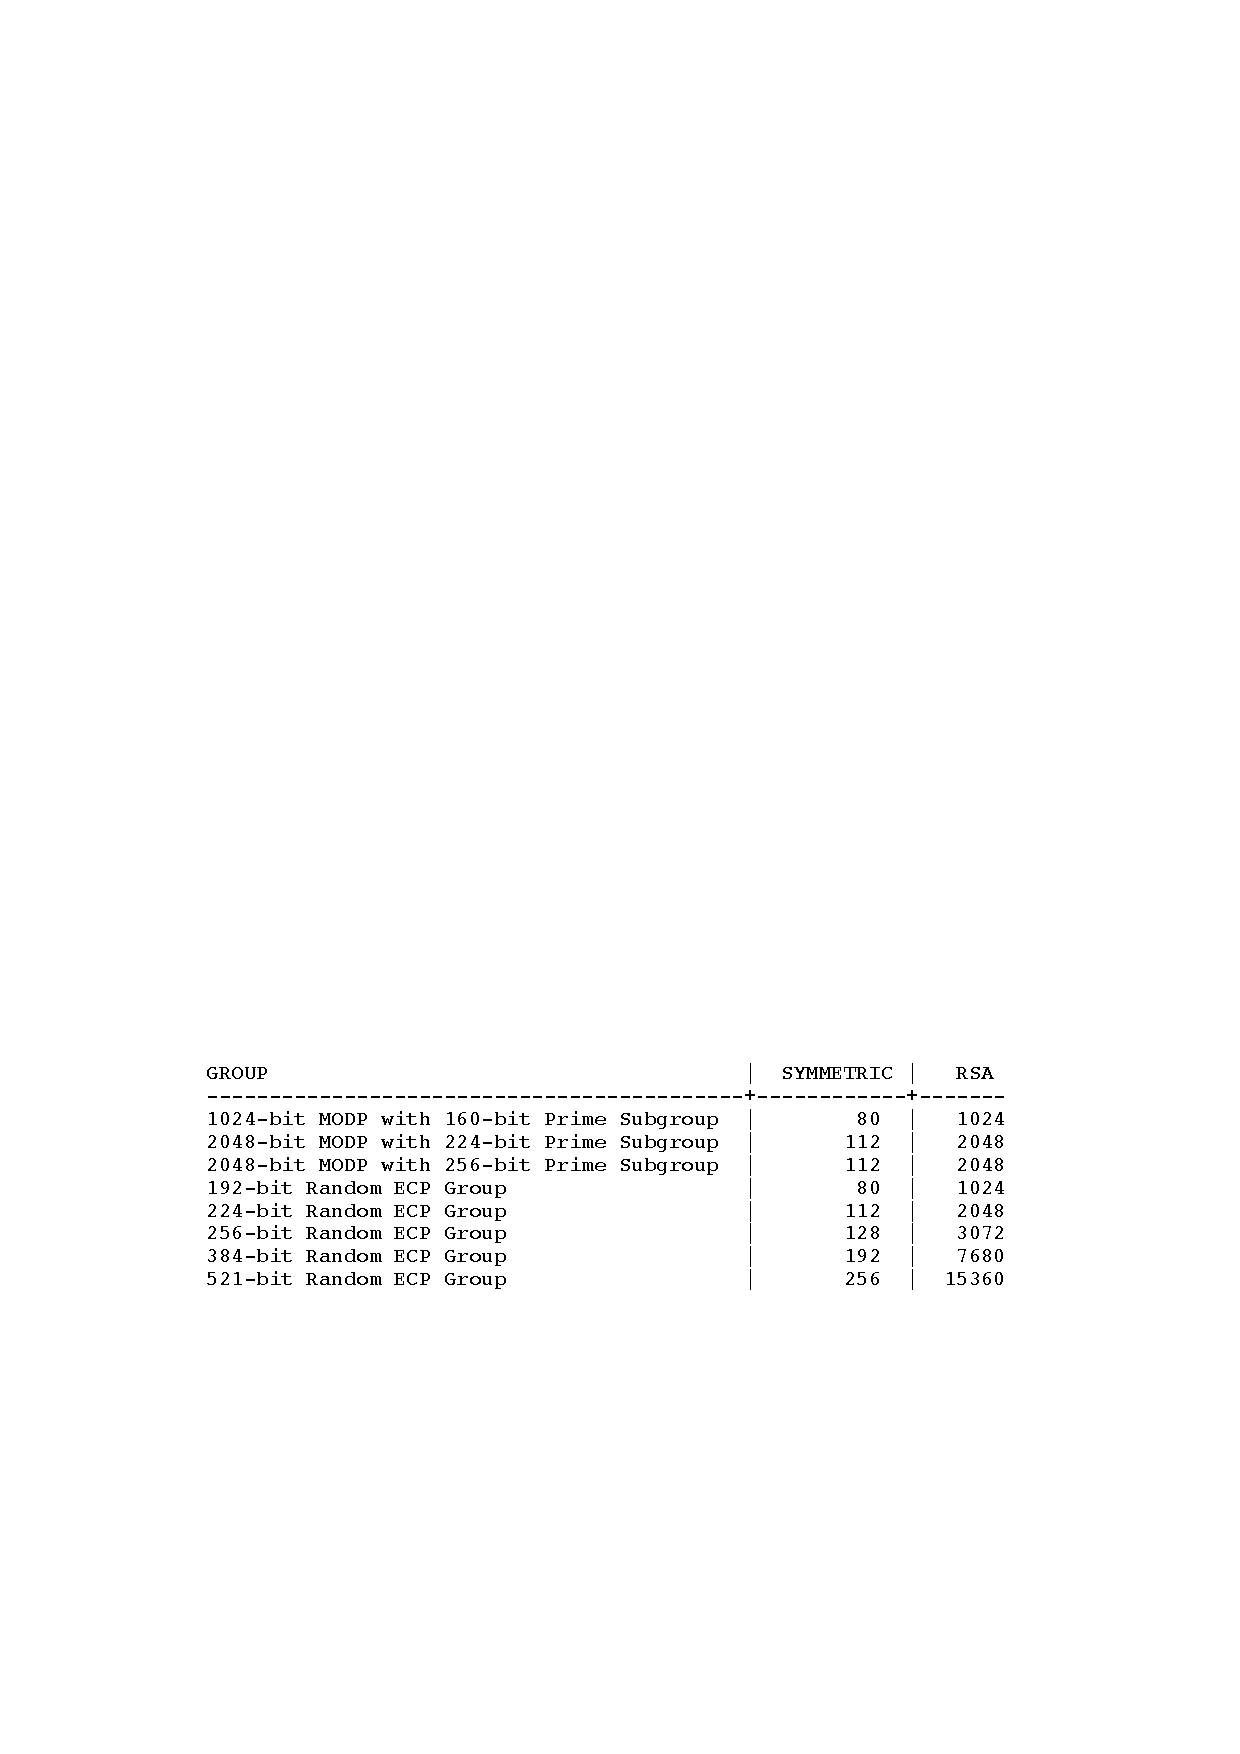
\includegraphics[width=1.0\textwidth]{rfc5114-security}
   \caption{In section 4, `Security Considerations', of RFC 5114\cite{rfc5114} the authors argue that ECC keys can be made much shorter without sacrificing security. Each line is cross-reference of different encryption types and key lengths offering the same cryptographic security. Notably, the benefits of ECC becomes even greater as the level of security is increased.}
   \label{fig:eccbenefits}
\end{figure}

In order to evaluate the possibilities of ECC in a resource constrained host, I decided that the IKEv2 implementation should implement the DH key exchange by means of ECC, using one of the shorter groups as seen in \vref{fig:eccbenefits}.


\paragraph{IKEv2 supports several authentication methods:} public key signatures, shared secrets and the Extensible Authentication Protocol (EAP)\cite{rfc3748}. As EAP is more complicated (i.e. higher complexity) than the other methods, I believe it's of no interest to this implementation and thus I will only focus on the former methods. Section 2.15 in RFC 5996 serves as a good introduction to the mechanisms used by the former methods (public key and shared secrets). What both schemes have in common is that they both perform a cryptographic operation on a string which is a concatenation of different IKEv2 messages and values shared by both parties\citep[p.48]{rfc5996}. (Please note that the formerly described DH key exchange only provides the hosts (peers) with a shared secret, not authentication. Thus, without any type of authentication, we're liable to a Man-In-The-Middle attack.)

The public key method (PKCS\#1) features the most flexibility and ease-of-use as it allows the peers to authenticate themselves using well known X.509 certificates, possibly using a public key infrastructure. Still, this method has not been implemented as it requires the implementation of digital signature algorithms\footnote{I had access to code that implemented digital signatures using Elliptic Curve Cryptography, but the work required to implement it with IKEv2 would have been far too large.}; handling the X.509 certificates; the certificate's payloads; etc. Not only would the required work effort be prohibitive, but the value of the work would be questionable as the extra asymmetric operation\footnote{We already perform one asymmetric operation during the DH key exchange} and the associated code itself would probably make it unpractical on current hardware. Still, it will certainly be practical on the future hardware reference platform that I define in \prettyref{sec:evalresults}.

Because of the aforementioned reasons, I have opted to implement the Shared Key authentication method as described in \citep[p.49]{rfc5996}. As it only requires the implementation of a simple pseudo-random hashing function (as described in section 2.13), the demands on ROM and CPU (and thus energy) are limited. The downside of this scheme is that it requires a string (the key) to be manually shared and maintained between the hosts that wishes to communicate. Although this gives rise an administrative hassle and arguably weaker security than the certificate alternative, it certainly affords security that's good enough for many situations.

% \paragraph{}
% As the purpose of this work is to demonstrate IKEv2 bla bla it has to be able to handle multiple sessions etc
% 
% The IKEv2 service is implemented as a Contiki Process.
% 
% The machine is built to be extended. The following is implemented as of now:
% 
% 
% Shared key auth. No X509. Simplified TS.
% Easily extendable to allow for missing features and other keying schemes for other applications.

\section{IKEv2 Implementation}
The IKEv2 implementation supports several concurrent sessions, each modeled as a mealy state machine\footnote{In a mealy state machine the output is function of the current state as well the current input, i.e. the output is a function of the transition.} that persists as long as the IKE SA is alive. As I will show, this enables communication with multiple hosts without excessive memory consumption.

\begin{figure}[h!]
   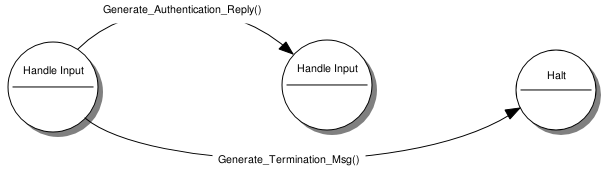
\includegraphics[width=1.0\textwidth]{fsm/mealy_demo}
   \caption{State machine example}
   \label{fig:mealydemo}
\end{figure}

As to begin the explanation, I would like to introduce the reader to the terminology used by the standard's document (RFC 5996 \cite{rfc5996}, hereafter referred to as `the RFC'). Therein, IKEv2 hosts are named \emph{peers} and their communications are called \emph{exchanges} consisting of a pair of \emph{messages}. There are four different types of exchanges, here displayed in order of usage during the lifetime of an IKE SA\footnote{An IKEv2 `session' (i.e. connection between two peers) are denoted as the IKE SA, which is the data structure containing the peer's shared cryptographic secrets.}: IKE\_SA\_INIT; IKE\_AUTH; CREATE\_CHILD\_SA; INFORMATIONAL. On the wire, each such message is an UDP datagram that begins the with the \emph{IKE header} and contains one or several \emph{IKE payloads}.

In the IKEv2 implementation, every \emph{message} is received by ike\_\-statem\_\-incoming\_\-data\_\-handler() which multiplexes the message on the basis of the unique identifier in the IKE header (the IKE SA's SPI). Each such SPI is associated with an IKE session and a corresponding state machine which represents that session's state. This determines what \emph{message} should go to which state machine instance.

In the state machine, each \emph{state} is represented by a function that, on the basis of the message received from the other peer, makes a \emph{decision} of how to act, i.e. what message to send in reply. That message is created and transmitted by its associated \emph{transition}, which itself is implemented as a function which only takes the session structure's pointer as its argument. This is a powerful feature of the implementation because it allows a message to be retransmitted without resorting to buffers storing the last transmitted message. Instead, the transition's function (whose pointer resides in the session struct) is simply run again. This saves several hundred bytes of RAM which otherwise would be required for buffer space. As the reply is received, the corresponding state function (determined by the session's data structure), is called and the process repeats.

The data structures and associated mechanism of the previously mentioned machines are interesting, but because of space constraints, they will not be reprinted here. Instead, the curious reader is directed towards the source code and machine.c and machine.h in particular.

% The rest of this section will be devoted to the description of the implementation of the IKEv2 protocol's responder and initiator machines.
Finally, before continuing with the description of the initiator machine, i would like to explain the terminology used for string processing. An example of such an operation is VAR = Ni | Nr. Here the variable VAR is assigned the value of the variable Ni concatenated with variable Nr. `N' is in this case an abbreviation of `Nonce' - a variable that exists at both of the peers, albeit with different values. Thus, `Ni' is the nonce of the initiator and `Nr' is the nonce the responder. This notation is commonly used throughout the standards document.


\subsection{Initiator machine}
An IKEv2 session is started or \emph{initiated} by one of the peers. The other peer that is contacted by the latter is then considered to be the \emph{responder}. The state machines for the two roles are slightly different, in the sense that the steps in the handshake process comes in a different order, but they are essentially the same and most of the source code are in common. This part describes the initiator machine, but it will allow you to understand the responder as well.

\begin{figure}[h]
   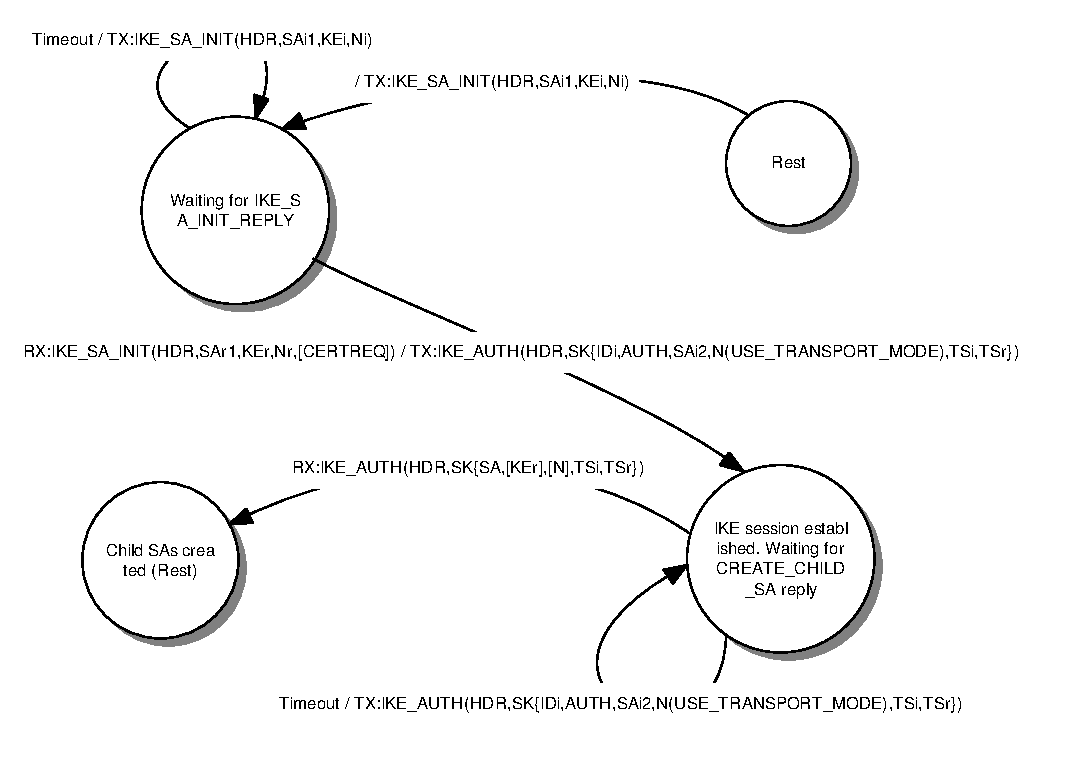
\includegraphics[width=1.0\textwidth]{fsm/initiator_mealy}
   \caption{The IKEv2 initiator's state machine}
   \label{fig:initiator-machine}
\end{figure}

An instance of the initiator machine is (as displayed in \prettyref{fig:initiator-machine}) is \textbf{started} when an application on the same Contiki host attempts to transmit a packet that matches the \emph{traffic selector} of an SPD rule labeled \emph{PROTECT} that has no matching SA. Now, the IKE session's data structure is setup by ike\_\-statem\_\-setup\_\-initiator\_\-session(ipsec\_addr\_t *triggering\_pkt\_addr, spd\_entry\_t *commanding\_entry) in machine.c. That data structure consists of two parts: one persistent and one ephemeral. The former contains the IKE SA (parameters, keying material used to derive subsequent child SAs and the IKE SA's authentication / integrity- and encryption keys); the remote peer's IP address; the IKE SPIs\footnote{Security Parameter Index, the IKEv2 session identifier}; data for connection house keeping such as message ID counters and retransmission timer; current state machine transition (i.e. the function that generated the last \emph{message}); target state (i.e. the function that should handle any \emph{responses} received in regard to the sent \emph{request}, or vice versa). The later (ephemeral) data structure stores information that is only of interest during the IKE session's setup: Pointer to the SPD entry that triggered the negotiation; storage for cryptographic nonces; storage for the peer's SA proposals; the private Diffie-Hellman key. Memory for both data structures are allocated with malloc(). In addition to this, the cryptographic nonce and the private key used in the Diffie-Hellman exchange is generated via a pseudo-random function. The reason that the private key is generated now and stored in the ephemeral data structure (to be thrown away after the handshake is complete) is that we lower the memory requirements, while key generation is comparably cheap energy-wise. Needless to say, this `trick' will have to abandoned is X.509 certificates or similar is to be used for authentication as the remote peer in that case expects a \emph{particular} private/public key pair, and not just anything\footnote{N.B. this implementation uses the pre-shared key method (\citep[p.49]{rfc5996}) for authentication.}.

\textbf{The first exchange, of type IKE\_SA\_INIT}, now begins when the state machine leaves the rest state and transmits the first message. The message consists of three payloads: the cryptographic offer for the IKE SA (i.e. suggested suite of integrity / authentication and encryption transforms); the peer's public Diffie-Hellman key; the cryptographic nonce that later one will be used for authentication the peers. It's also at this point that the public key is computed, something which takes considerable time (see \prettyref{cha:eval}).

The state machine is now in state \#2 and \textbf{waits for the peer's reply}, a message containing the very same payloads that we just sent. If the peer accepted our IKE SA offer, the SA payload will now contain the peer's choice of cryptographic transforms, a subset of our previous offer. Likewise, if the peer found our choice of asymmetric algorithm acceptable, the KE payload will contain the peer's public key calculated for the same parameters\footnote{A Diffie-Hellman key exchange's cryptographic transform is determined by its IKE DH group, in IKEv2 parlance.}. Both peers now have a shared Diffie-Hellman secret and can thus form an IKE SA using the secret as the source of keying material. This is done in the following way:

\begin{figure}[h]
   \begin{verbatim}
SKEYSEED = prf(Ni | Nr, g^ir) 
{SK_d | SK_ai | SK_ar | SK_ei | SK_er | SK_pi | SK_pr } =
   prf+ (SKEYSEED, Ni | Nr | SPIi | SPIr )
   \end{verbatim}
   \caption{Deriving keys for the IKE SA and keying material for future Child SAs. $g^{ir}$ is the shared Diffie-Hellman secret. N* strings are the responder's and the initiator's nonce strings; SPI* are the IKE SA's SPIs numbers (used for identification); SK\_a* and SK\_e* is the IKE SAs cryptographic keys; SK\_d is a string from which keying material can be derived for future child SAs (hence `child' in the sense that it inherits keying material from a parent SA); SK\_p* is material that will be used for authenticating the peers during the IKE\_AUTH exchange. The functions prf and prf+ are described in \prettyref{fig:prf}.}
\end{figure}


\begin{figure}[h]
   \begin{verbatim}
      prf = HMAC (Key, String) 
      
      prf+ (K,S) = T1 | T2 | T3 | T4 | ...
      T1 = prf (K, S | 0x01)
      T2 = prf (K, T1 | S | 0x02)
      T3 = prf (K, T2 | S | 0x03)
      T4 = prf (K, T3 | S | 0x04)
   \end{verbatim}
   \caption[The functions prf and prf+]{The prf function is an HMAC-function and is negotiated during the IKE\_SA\_INIT exchange. This implementation uses HMAC-SHA1 exclusively. The utility of the prf+ function is the ability to generate strings of keying material of any length i.e. regardless of the prf function's output. The prf+ function is defined on p.46 in the RFC.) }
   \label{fig:prf}
\end{figure}

The IKE\_SA allows the peers to communicate securely, but only if the risk of a possible man-in-the-middle attack is discounted. This will be remedied in the next exchange, IKE\_AUTH, which will authenticate the peers.

Given that we can parse the peer's message without trouble, \textbf{the state machine transmits the first message of the IKE\_AUTH exchange} by transiting to the next state. This message consists of one encapsulating payload which encrypts the others using the IKE SA. Its structure is almost identical to that of the ESP header, which allowed me to implement the encoding and decoding of these two payloads / headers in the same C-function. The encapsulated payloads are: ID (an e-mail address - one of seven different ID methods); Authentication data (AUTH); an offer of cryptographic transforms for the child SA pair (i.e. the SAs that will be used by IPsec); Notification payload that informs the other peer that only Child SAs for IPsec transport mode are acceptable; Traffic Selectors - one for each direction of the traffic flow that the Child SAs will carry.

As previously stated, IKEv2 can use both digital signatures as well as shared keys, this implementation making use of the latter. In common to both methods is that their authentication data is based upon a signature or hash of the string in \prettyref{fig:sign-string}.

\begin{figure}[h]
\begin{verbatim}
InitiatorSignedOctets = RealMessage1 | NonceRData | MACedIDForI
GenIKEHDR = [ four octets 0 if using port 4500 ] | RealIKEHDR 
RealIKEHDR = SPIi | SPIr | . . . | Length 
RealMessage1 = RealIKEHDR | RestOfMessage1
NonceRPayload = PayloadHeader | NonceRData
InitiatorIDPayload = PayloadHeader | RestOfInitIDPayload 
RestOfInitIDPayload = IDType | RESERVED | InitIDData 
MACedIDForI = prf(SK_pi, RestOfInitIDPayload)
\end{verbatim}
\label{fig:sign-string}
\caption{The string to be signed is a concatenation of the peer's nonces; previously transmitted messages and more.}
\end{figure}

The fact that the string described in \prettyref{fig:sign-string} includes previously transmitted messages (RealMessage1) incurs an extra memory overhead as the messages needs to be buffered. In this implementation I partly alleviate this problem by only buffering the remote peer's message. The peer's own message is reproduced by simply re-running the transition associated with the message in question.

\begin{figure}[h]
\begin{verbatim}
AUTH = prf( prf(Shared Secret, "Key Pad for IKEv2"),
<InitiatorSignedOctets>)
\end{verbatim}
\label{fig:final-sign}
\caption{Computing authentication data using the shared secret method. From p.49 RFC 5996.}
\end{figure}

Finally, using the shared secret authentication method, the authentication data for the AUTH payload is computed as seen in \prettyref{fig:final-sign}.

The traffic selectors are used for negotiating what kind of IP packets that can be transported across the child SA. The initiator's role is to negotiate a traffic set (traffic selector) that resembles the SPD rule that triggered the handshake as closely as possible. The responder will try to be as accommodating as possible, but might reply with only a subset\footnote{This is referred to as `narrowing' in the RFC.} of the initiator's traffic set in order to not violate its own policy. In the worst case the two peers' SPD configurations are inherently incompatible and the traffic negotiation will fail, causing the creation of the child SA to be abandoned.

The implementation constructs a set of traffic selectors that are in compliance with the standard: the first selector pair have the same address parameters as that of the triggering packet (i.e. the same IP address, the same ports etc); the second is a copy of the triggering SPD rule, but the rule's IP address range is replaced with the IP of the peer\footnote{The RFC refers to such address replacement as Populate-From-Packet (PFP). It also dictates that the administrator should be able to set a PFP flag for each one of the fields in the address selector, but I ignored that and hardcoded the PFP flag for the address field.}.

\textbf{The state machine now expects an IKE\_AUTH reply from the peer.} Just as with the IKE\_SA\_INIT exchange, we expect to see the same payloads in return: The peer's ID; peer's authentication data; child SA transform reply; traffic selector reply.

The authentication data is re-computed, but using the peer's values instead, according to the procedure in \prettyref{fig:sign-string} and \prettyref{fig:final-sign}. If the computed value corresponds to that in the received AUTH payload, we can be certain that the peer that we share the IKE SA with is also in possession of the \emph{shared secret} referred to in \prettyref{fig:final.sign}.

With authentication complete, the state machine can now create the child SAs (each being half-duplex with respect to traffic flow). The child SA transform (encryption, intergrity and authentication settings) reply is expected to be a subset of that we sent to the peer, if it found it acceptable. If the transform set is indeed a subset of the offer, the transforms are accepted. The corresponding procedure is carried out for the traffic selector set: the reply is accepted if it's a subset of the offer.

\begin{figure}[h]
\centering
\begin{verbatim}
KEYMAT = prf+(SK_d, Ni | Nr)
\end{verbatim}
\label{fig:child-keymat}
\caption{Creating keying material for the Child SAs.}
%. Perfect Forward Secrecy is achieved by feeding the material through a HMAC-function (prf+).}
\end{figure}

The keys for the cryptographic transforms of both Child SAs are taken from the KEYMAT string in the order described on page p.52 of the RFC. The SAs are now inserted into the SAD and the state machine frees up the ephemeral data structures. The IKE SA is retained for future use, but may be terminated if memory if so wished.

\subsection{Responder machine}
The responder shares almost all of its code with the initiator. What sets them apart is the order by which strings are concatenated (e.g. consider Ni | Nr) and the structure of the state machine.

 % As the responder The latter has implications for memory management: The responder can always access the initiator's packet in Contiki's IP packet buffer and therefore doesn't need to buffer . where the responder has access to the packet's data just received from the initiator while the latter has to buffer them for computations done at a later stage.

\begin{figure}[h]
   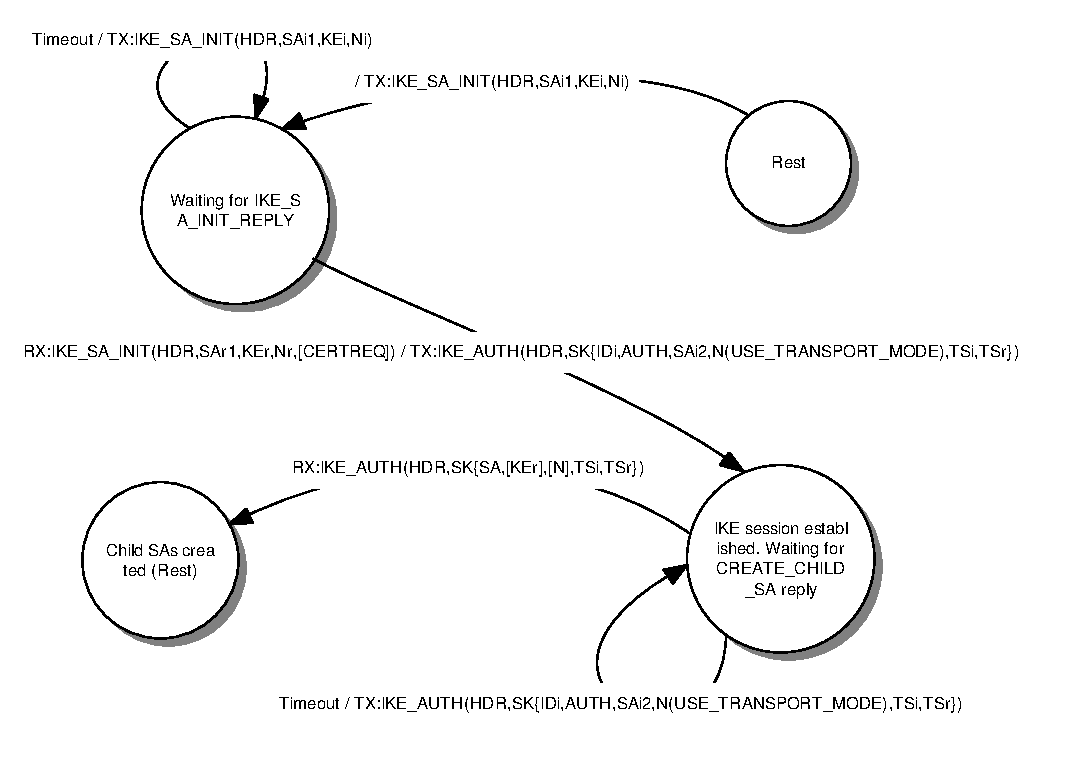
\includegraphics[width=1.0\textwidth]{fsm/responder_mealy}
   \caption{The IKEv2 responder's state machine}
   \label{fig:responder-machine}
\end{figure}

\section{Supporting libraries}
The suite makes use of several cryptographic algorithms e.g. SHA1, HMAC, AES, etc. This functionality is provided to the software suite in the shape of libraries provided by other authors. These are written with the explicit purpose of being performance-efficient and are therefore well suited to this project. Here follows a list of the libraries used and their contribution to the suite:

\paragraph{ContikiECC} is my port of TinyECC, a library for asymmetric encryption using elliptic curves (ECC) originally created for TinyOS. It contains a multiple precision arithmetic library upon which elliptic curve encryption functions are implemented. These are used by IKEv2's Diffie-Hellman key exchange. Support for ECC-based Digital Signatures, which can be used for X.509 certificates, is also implemented, but is not used by the IKEv2 service.

\paragraph{The AES encryption standard} is implemented in software. Previous IPsec implementations\cite{raza11securing} have made use of hardware implementations, but this was not possible as the radio module that provided the functionality in question was not part of the chosen development platform (Wismote, see \prettyref{cha:eval}). The library in question is a part of the popular MIRACL SDK.

\paragraph{The HMAC-SHA1-96 standard} as defined in RFC 2104\cite{rfc2104}, is used by IPsec as an integrity/authentication mechanism (see RFC 2404\cite{rfc2404}), and by IKEv2. The HMAC implementation is also a part of the MIRACL SDK, but I altered it in such a way that it could utilize ContikiECC's SHA1 implementation.


\chapter{Evaluation}
\label{cha:eval}
The software was evaluated using the Cooja emulator as stated in \prettyref{sec:finaldev}. The emulated mote (Wismote) features a 16 bit CPU with an instruction set (MSP430x) that includes instructions for 20 bit memory operations and runs at 16 MHz. There is 16 kB RAM and 128 kB of flash (for storing program data). Usually IoT application like this is evaluated on the Tmote Sky platform, but as I will soon show you, its 16 bit memory space is too limited (keep in mind that the RAM and flash area occupies the same $2^16$ address space).

The other peer consisted of Cooja's host using the Linux kernel's native IPsec implementation and the Strongswan software suite for providing the IKEv2 services.

\section{IPsec implementation coverage}
The IPsec part of this implementation should be, to the best of the author's knowledge, compliant with all relevant standards with the exception of certain features (see \prettyref{sec:ipsec-features-not-imp}).

\subsection{Major features implemented}
\begin{itemize}
   \item Packet replay protection
   \item The ESP header
   \item IPsec Transport mode
   \item Traffic selectors (traffic multiplexing over SAs)
   \item SAD, with mechanism for SA expiration
   \item SPD and related functions (including one SA offer for each SPD rule)
   \item Confidentiality protection (Encryption): 
   \begin{itemize}
      \item ESP-NULL
      \item AES-CTR, varying key length (only 128 bit tested). This was a partial rewrite of Simon Duquennoy's code.
   \end{itemize}
   \item Integrity protection:
   \begin{itemize}
           \item AES-XCBC. This was a partial rewrite of Simon Duquennoy's code.
   \end{itemize}
\end{itemize}

\subsection{Major features not implemented}
\label{sec:ipsec-features-not-imp}
\begin{itemize}
        \item The AH header
        \item IPsec Tunnel mode
        \item Various integrity and encryption algorithms that the standards document regards as required.
\end{itemize}

The lack of support for the AH header and tunnel mode is of no consequence for reasons as described in \prettyref{para:ah-not-impl} and \prettyref{para:tunnel-mode-not-impl}, respectively. The lack of support for encryption transforms other than AES-CTR and AES-XCBC can be hampering to interoperability, but this IPsec implementation is fashioned in such a way that new transforms can be implemented with ease.

\section{IKEv2 implementation coverage}
\label{sec:ike-impl-coverage}
The IKEv2 implementation is a subset of the standard described by RFC 5996. It's not standards compliant because of missing features.

\subsection{Major features implemented}
\begin{itemize}
   \item State machine for responder
   \item State machine for initiator
   \item ECC DH (only featuring support for DH group no. 25)
   \item Authentication by means of a pre-shared key
   \item Traffic selector negotiation (only a simplification of \citep{rfc5996}[section 2.9]'s algorithm)
   \item SPD interface that allows multiple IKE SA offers
   \item SK payload: Code for encryption and integrity is shared with IPsec's ESP
   \item Multiple concurrent sessions supported
   \item Multiple child SAs per IKE SA
\end{itemize}

\subsection{Major features not implemented}
\begin{itemize}
   \item Cookie handling (the code has been written, but it has not been tested)
   \item Only tunnel mode negotiation supported
   \item No EAP support
   \item No NAT support
   \item No IPcomp support
   \item Only IDs of type ID\_RFC822\_ADDR (e-mail address) are supported
   \item No support for Certificates as IDs, nor for authentication
   \item No state machine for established sessions
\end{itemize}

The established state machine was not implemented because of time constraints, but doing so would be a straightforward task and would not require any changes to the architecture of the software. This resulted in that the IKEv2 service doesn't recognize the Delete Payload and thus cannot delete SAs, nor can new Child SAs be created.

%Features that should be implemented in IKEv2, but haven't yet:
% Deletion of Child and IKE SAs (Delete payload)
% State machine Established can't create child SAs currently


\section{Test setup}
\label{sec:test-setup}
The software can be configured to be built with different feature sets so that the developer can reduce the resource requirement. This gives rise to a large number of feature-sets that can be evaluated. In order to reduce the size of the investigation to manageable proportions, I have elected to limit myself to the two most important configurations:

\begin{itemize}
   \item IPsec with manual keying and a test application that replies to UDP packets. Henceforth named NOIKE.
   \item IPsec with automatic keying only, IKEv2 and a test application that replies to UDP packets. Henceforth named WITHIKE.
\end{itemize}

NOIKE's SAs were configured to use AES-XCBC-MAC-96\cite{rfc3566} for integrity / authentication and AES-CTR\cite{rfc3686} for confidentiality. The key length of the latter was 128 bits.

The IKEv2 offer of the WITHIKE system was set up in such a way that it and its peer negotiated SAs of the same configuration as that of the NOIKE system. The handshake was triggered by the PC by attempting to transmit a UDP packet (using the \emph{nc} utility) from the PC to the mote using a port that was configured for protection. That caused Strongswan's \emph{charon} demon initiated a key exchange with the mote's IKEv2 service (making use of the IKEv2 service's responder state machine). The key exchange used $192$ bit ECC keys (the curve is named secp192r1 as described in `Additional Diffie-Hellman Groups for Use with IETF Standards' in RFC 5114\citep[p.5]{rfc5114}). Its security level is deemed to be comparable to that of a symmetric encryption scheme with a key length of 80 bits\citep[p.11]{rfc5114}. A shared secret was used for authentication as this is the only type of authentication implemented in the service as of today.

\section{ROM and RAM requirements}
\label{imagecomp}
The image's ROM requirement was determined using the following method.

\begin{quotation}
A `bare' Contiki system is compiled (i.e. one without IPsec) and the image named contiki-bare; Another Contiki image with the feature in question included was then compiled and named in the style of contiki-FeatureName; the size of of the two images' segments are now compared with a suitable tool such as `size'. The three segments are listed here with their usual members\footnote{There is nothing in the specifications for the C language that stipulate where certain language constructs should be stored in the resulting image. For example, constants are usually stored in the text segment, but we cannot be certain without reading the compiler's documentation.}: Data (initialized variables), BSS (uninitialized variables) and Text (Program code and constants).

All code was compiled with MSPGCC 4.7.2 without debug symbols and using the optimization flag Os which emphasizes text segment reduction over execution speed (e.g. limited loop unrolling). Debug symbols and diagnostic messages have been excluded from the image.
\end{quotation}

This resulted in the following figures for a default Contiki system (i.e. no IPsec / IKEv2 features), NOIKE and WITHIKE, respectively:

\begin{figure}[h]
\begin{verbatim}
    text	   data	    bss	    dec	filename
   55734	    264	   9310	  65308	manualsa-noike.wismote
   47502	    252	   8960	  56714	noipsec.wismote
   74241	    288	   9582	  84111	nomanualsa-ike.wismote
\end{verbatim}
\caption{Raw figures for ROM and RAM requirements as given by the `size' command.}
\end{figure}


% 54,685546875 9,349609375
% 46,634765625 8,99609375
% 72,7822265625   9,638671875

\begin{figure}[h]
\begin{tabular}{c|l|l}
Configuration                          & ROM (text + data)        & RAM (data + BSS)            \\ \hline
default (Contiki with $\mu$IP6)        & 46.6 kB                  & 9.0 kB                      \\
NOIKE                                  & 54.7 ($\Delta8.1$) kB    & 9.4 ($\Delta0.4$) kB        \\
WITHIKE                                & 72.8 ($\Delta26.2$) kB   & 9.6 ($\Delta0.6$) kB
\end{tabular}
\label{tab:rom-ram-eval}
\caption{ROM and RAM requirements, with size difference relative to the default configuration noted.}
\end{figure}

% Det är normalt att bss är mycket större än data. bss är oinitialiserat minne som t ex granntabeller, paketbuffrar, etc. medan data är initialiserat minne vars värden kopieras upp från flash vid boot (tex "static int v = 47;").
% 
% Totalt använt flash ~= text + data
% Totalt använt minne ~= data + bss

%#################

% This gives an image size (ROM size) of ~8 kB for the case of IPsec with manual keying. 
% In the case of IPsec with manual keying
% 
% That's probably the best choice as Simon's code is undoubtedly smaller since it's more specific. It also features support for offloading the AES operations to the CC2420 radio, while I am doing it in software.
% 
% I've fixed the build problems now, but my implementation still requires ~8 kB if dynamic key management is excluded. Inspection of the binary reveals that the AES implementation represents ~2.5 kB of that sum. Thus, the grand total could probably be squeezed down to 5-6 kB, but it's still quite hefty for a small Tmote Sky.
% 
% In total, with dynamic key management, the code's size is 26,5 kB.
% 
% All measurements are without debugging symbols and messages.


% Different types of RAM req.: stack vs global vars

\section{Stack requirements}
\paragraph{If the stack grows to large} it will overwrite the heap or simply exit the RAM's memory area. Therefore, we want to know its maximum extent in different situations.

The stack requirements for the NOIKE configuration have not been measured as they are considered very limited - probably not more than 100 B. This can be assumed by the fact that the IPsec source code 1) is not deeply nested (i.e. depth of the function calls) 2) there are no large variables in those function calls. 

%Furthermore, the source code in question is only executed during the course of the transmission or reception of an IP packet. I.e. the stack allocation has been freed once the $\mu$IP code exits.

However, the stack requirements of the WITHIKE configuration are extensive because of the IKEv2 service's need to 1) concatenate large strings in order to compute their hashes 2) perform asymmetric encryption operations. Therefore we will only investigate the stack usage of the WITHIKE option.

\paragraph{The size of the stack was measured by} writing a 2 kB long string consisting of the letter `h' to the top of the stack before commencing the IKEv2 handshake. That string's memory was then investigated after the handshake to see what parts had been overwritten by the service's handshake routines:

\begin{figure}[h]
\centering
\begin{verbatim}
for ( i = STACK_MAX_MEM - 5;
      i > 4 && strncmp((const char *) (buff + i), "hhhhh", 5);
      i -= 1)
      ;
\end{verbatim}
\label{code:stack}
\caption{STACK\_MAX\_MEM is set to 2 kB and the pointer \emph{buff} point to the string. Because the stack extends downwards on the MSP430 architecture, the loop starts investigating the end of the string as it's closest to the rest of the stack. It exits when it finds the `h' pattern.}
\end{figure}

The maximum extent of the stack during the handshake was found to be 320 Bytes according to this method.

\begin{figure}[h]
\centering
\label{tab:eval-stack}
\begin{tabular}{c|l}
Exchange                      & Maximum extent of stack  \\ \hline
IKE\_SA\_INIT exchange      & $321$ B                    \\
IKE\_AUTH exchange          & $203$ B                    \\
After handshake            & Not applicable
\end{tabular}
\caption{Maximum extent of the stack at different times during the key exchange.}
\end{figure}

\section{Heap requirements}
The use of heap allocation is not customary in Contiki - fixed buffers are used instead. However, I elected to use the heap (by making use of the \emph{malloc} call) in the IPsec as well as the IKEv2 code as the memory requirements varies extensively by activity.

The memory usage was traced by creating a wrapper function around the call to \emph{malloc} and \emph{free} that kept statistics on memory allocation. This resulted in the following memory pattern for the node when acting as the IKEv2 responder:


\begin{figure}[h]
\centering
\label{tab:eval-heap}
\begin{tabular}{c|l}
Exchange                      & Maximum amount of heap memory allocated    \\ \hline
IKE\_SA\_INIT exchange        & 930 B                                      \\
IKE\_AUTH exchange            & 1142 B                                     \\
After handshake               & 402 B
\end{tabular}
\caption{Maximum size of the heap at different times during the key exchange.}
\end{figure}

Of the remaining memory, $2 * 106 B$ is used for the SAs\footnote{Keep in mind that IPsec requires one SA for each direction} and 190 B is consumed by the IKE SA. If more SAs are created using this IKE SA, the memory consumption would increase on the order of $2 * 106 B$ per duplex connection.
% 
% \begin{tabular}{c|l|l|l}
% Exchange                   & CPU Time consumed  & Maximum extent of stack  & Allocated memory on the heap   \\ \hline
% IKE\_SA\_INIT exchange       & 6.91 s             & 320 B                    & 930 B                          \\
% IKE\_AUTH exchange          & 3.97 s             & 210 B                    & 1142 B                         \\
% Final                      & 10.87 s            & n/a                      & 402 B
% \end{tabular}

\section{Latency}
The CPU time consumed by the IKEv2 service during a key exchange is 10.9 seconds when run on the Wismote. This excludes the time required to transmit the messages and the other peer's delay. The total time (i.e. clock time) for a key exchange is 11.1 seconds. That includes message transmission time as well as the delay caused by the other peer.

\begin{figure}[h]
\centering
\begin{tabular}{c|l}                        
Exchange                   & CPU Time consumed     \\ \hline
IKE\_SA\_INIT exchange     & 6.91 s                \\
IKE\_AUTH exchange         & 3.97 s                \\
Total                      & 10.87 s            
\end{tabular}                                   
\caption{Time requirements for the different phases of the key exchange.}
\end{figure}

\label{sec:latency-similar}
The latency / CPU time associated with the NOIKE option was not investigated as the bulk of its execution time is spent in code  that is virtually the same as the one found in \cite{raza11securing} (the code in question concerns cryptographic operations). The paper in question features a number of investigations covering latency and energy usage of the code concerned.

%* IPsec packet: Energy required for receiving, energy required for transmitting. Roundtrip times. 
%IPsec packet: See Shahid's paper. Should be very similar. CC2420 crypt?

\section{IKEv2 total RAM consumption at different times}
\label{sec:eval-sum}
The RAM consumption of the IKEv2 service is changing as the system boots; SAs are established; and the service returns to an idle state. Investigating these figures allows us to understand how much memory that is left for applications at different times.

\begin{figure}[h]
\centering
\begin{tabular}{ p{2.25cm} | l | p{2.25cm} | p{2.25cm} | p{2.25cm} }                        
State                   & $BSS + data$ & Max. extent of stack  & Max. extent of heap   & Total Maximum  \\ \hline
After boot up           & 9.6 kB       & 0 kB                  & 0 kB                  & 9.6 kB       \\
IKE\_SA\_INIT exchange  & 9.6 kB       & 321 B                 & 930 B                 & 10.9 kB      \\
IKE\_AUTH exchange      & 9.6 kB       & 203 B                 & 1142 B                & 11.0 kB      \\
Est. SA pair and IKE-SA & 9.6 kB       & 0 B                   & 402 B                 & 10.0 kB      \\
Est. SA pair            & 9.6 kB       & 0 B                   & 212 B                 & 9.9 kB
\end{tabular}
\caption{The data in the table is based up the figures presented above. The second column is the size requirement of the image, the second and third is memory used by IKEv2 dynamically, and the fourth is the sum of the memory used by IKEv2 at the current phase. The sums are recomputed from the original, non-rounded, size measurements.}
%`RAM used' is the sum of the image's \emph{data}- and \emph{BSS}-area and the current size of the \emph{Stack} and \emph{Heap}.}
\end{figure}

This reveals that the maximum memory usage of the IKEv2 service occurs during IKE\_AUTH exchange and amounts to 11 kB. It should be mentioned that 203 of those bytes is used by the IKEv2 process's stack and are available for use by other processes' stacks, but subtracting the values in the column `Total Maximum' from the total available RAM memory\footnote{Which is 16 kB in the case of the Wismote platform.} gives the maximum amount of memory that other processes safely can use. Finally, another 190 bytes can be freed if the IKE session (IKE SA) is destroyed after creation of the two child SAs. This is currently not done and would require a new set of IKE\_SA\_INIT, IKE\_AUTH exchanges if the negotiation of new SAs would be required.  


\section{Source code complexity}
A common way of measuring source code complexity is by the number of lines of source code (commonly abbreviated as SLOC). Counting the number of of lines of code; including comments, but excluding blank lines; the full software suite (IPsec + IKEv2) encompass $11 764$ lines of C source code. If comments are excluded, the number of lines becomes $5 985$.

Of those $11 764$ lines, $3 801$ lines (code as well as comments) are consumed by the support library ContikiECC (unused elliptic curves and features are not included in the figure) and the HMAC implementation. The various IPsec transforms (AES-CTR etc) and the supporting AES implementation are not included in this figure.

Out of the total $11 764$ lines, $7 109$ lines (approximately $3 200$ lines if excluding comments) is the exclusive work of the author. In addition to this, my work also consisted of: adaption of TinyECC (written for TinyOS originally) for Contiki, forming what I named `ContikiECC'; key parts of the HMAC-SHA1-96 implementation was changed in such a way that it could make use of ContikiECC's SHA1-implementation in order to save memory; the implementation of IPsec's transforms were re-written in a number of ways in order to interface with the rest of the IPsec stack and improve clarity.




\chapter{Discussion}
In this chapter I will discuss the results described above and the methodologies used in gathering them.

\section{Evaluation method}
In addition to demonstrating the usability of the implementation (i.e management of SAs), the primary concern of the evaluation was measuring ROM and RAM consumption as well as CPU requirements (i.e. latency).

\subsection{IPsec}
The evaluation demonstrated the automatic negotiation of SAs, a test which also covered the basic working of the SAD, the SPD and the rest of the IPsec system. The author believes that these result are easy to reproduce in other conditions with different network configurations and Contiki applications of different communication patterns. This is especially true of the IPsec system which encompass header generation and parsing (the $\mu$IP6 implementation), the SPD and the SAD, where the implementation should be complete and therefore have a high degree of interoperability.

\subsection{IKEv2}
The evaluation of the IKEv2 system only covered portions of what the standards documents considers mandatory for an implementation. The reason for this is twofold: the minimalistic implementation (i.e. lack of features to be tested) and the time required for configuring, testing and writing more test. The biggest downfall of this was the lack of testing of the traffic selector negotiation, whose algorithm is a simplification of that described in the standards documents. The author is not sure how it will function when negotiating other SPD offers\footnote{Please remember that the SPD offer for different SPD policies is configured by the peer's administrator.} with peers running other IKEv2 implementations than Strongswan.

\subsection{ROM and RAM measurement}
The evaluation of the image's ROM and RAM usage was straightforward and the numbers should be correct, caveat the following: the test application's (the UDP message `bouncer') was included in all images of \prettyref{tab:rom-ram-eval}; no status, nor any error message strings were included in the binary, making in-field diagnostics difficult.

Stack and heap measurement figures should be correct to the byte by virtue of the evaluation techniques described in \prettyref{cha:eval}.

\subsection{Time}
Time / latency testing was only performed on the Wismote platform as it was, arguably, the weakest platform that could comfortably accommodate the software. The rationale of that decision is that by ascertaining the functionality of the software on a simple platform, it can be assumed that it will work better on more powerful ones.

The time required for an IKEv2 handshake is heavily dependent upon the key length of the asymmetric key as it's completely dominated (more than 80\%) by ContikiECC's large-number integer arithmetic.

% Diskutera mina resultat: Styrkor och svagheter i vad gäller undersökningsmetodiken

\section{Evaluation results}
\label{sec:evalresults}
Previous publications\cite{raza11securing} have shown that IPsec is feasible on Contiki. In \prettyref{cha:eval} of this thesis I show that IPsec with IKEv2 for automated SA management is feasible, at least on the coming generation of 32 bit hardware. In \emph{this section} I will present the reasoning behind the statement by discussing the software's performance on the current Wismote platform and improvements to be expected on future platforms.

With the purpose of making the discussion clearer I have elected to discuss future hardware in terms of a reference platform of my choice, namely STM32W from STMicroelectronics, which Contiki has been ported to. It's an ARM Cortex M3 based platform featuring an embedded IEEE 802.15.4 radio, up to 16 kB and 256 kB of RAM and flash memory (ROM), respectively. There are many reasons to expect hardware like this to become the mainstay of IoT nodes in the near future, but the chief one is that these MCUs are becoming more power-efficient\cite{ko2012low} (in per-instruction as well as in sleep-mode power consumption) than the (in the world of IoT) hitherto incumbent line of 8- and 16-bit devices.

The investigation of the feasibility of IPsec/IKEv2 (or any other network protocol for that matter) on Contiki begins by determining the ROM and RAM requirements of the protocol's implementation. Subsequently, it must be asserted that there is enough resources left for the typical application using the service. This is not a problem on the Wismote platform, which has 6 kB of RAM and 55 kB of ROM to spare after the IPsec/IKEv2 system has established an SA pair (see \prettyref{sec:eval-sum}). On the future reference platform, these margins will become plentiful.

However, feasibility is not achieved by simply fulfilling the memory requirements. It must be \emph{usable} as well i.e. operate in its environment completing its intended functionality. For IPsec/IKEv2 this translates into the following criteria: are the \emph{communication delays} with other peers tolerable (IKEv2); \emph{energy usage} (both); can the \emph{interoperability}\footnote{In this context, interoperability is defined as the ability to communicate with other peers.} be deemed passable? I will herein only discuss IPsec in the context of interoperability, as the other aspects have been conclusively covered in \cite{raza11securing}, which features a very similar implementation (discussed in \prettyref{sec:latency-similar}).

\paragraph{Interoperability} is perhaps the hardest problem to tackle. Beginning with IPsec: interoperability should be good enough for communication with any system, with the exception of those that 1) have specific requirements concerning cryptographic standards 2) requires IPsec tunnel mode. I can see no reason as to why such requirements should be anything other than exceptions.

The IKEv2 service requires, just like the IPsec system, that the peer that it's talking to is configured to only use the features and configuration sets that it understands. I do not anticipate this to be a problem when the peer can be configured for the Contiki system's needs, but if this is not possible, the results are uncertain. Hence, I am of the opinion that the IKEv2 service is usable if the peers' administrators are willing to adapt the configuration to the needs of Contiki.

(At this point I would like to remind the reader that the aspect of administrative intervention which the previous subject touches upon is applicable to IKEv2 as well as IPsec, while the opposite, the case of non-intervention on the behalf of a human, is not applicable to IPsec as that always requires human action for setup.)

%% In order to make the IKEv2 
%% IKEv2's interoperability is not certain, as its functions has not been evaluated any further than the test described in \prettyref{sec:test-setup}. 

%%Continuing with IKEv2. %FORTSÄTT HÄR

\paragraph{The energy usage} of the IKEv2 implementation has not been explored, but can be approximated from the time required for running the computations as those vastly exceeds the energy required for the associated transmissions. The corollary of this is that the question of energy consumption is determined by the algorithm used for the Diffie-Hellman exchange. As discussed in \prettyref{sec:ecc-improvements}, large improvements can be made by employing optimizations.

\paragraph{Communication delays} (the time required for to setup an SA pair with an hitherto not contacted client) amounts to slightly less than 11 seconds. This is definitely acceptable for most other IKEv2 peers in the sense that the delay won't cause\footnote{As an example, the default timeout for Strongswan's IKEv2 daemon \emph{charon} is 120 seconds.} a timeout / retransmission, and is probably also enough for most application's demands given that the SA can be established prior to actual usage. In the future reference platform, the time required by the key exchange will be on the order of four times as fast if we assume a clock speed of 32 MHz. The speedup is a result of not only clock speed, but also of an increase in word length from 16 to 32 bit, which will reduce the multiple precision library's operations by half.


% On the current reference platform (Wismote), the time required for a handshake (almost 11 seconds), is not long enough to cause timeout problems with other peers. The time requirements for 
% 
% The question of energy consumption was not explored as I didn't find 
% 
% Knowing that there is \emph{enough memory to run the suite} begs the question if the IPsec/IKEv2 implementation is \emph{practical} as well. That is, are the delays incurred by negotiation, the configuration 
% 
% Knowing that the software can be executed on the given hardware, we can focus on `softer' aspects such as delays and energy usage. As
% 
% The memory figures and processing speed will be on a 32 bit CPU; plenty enough.
% 
% Diskutera mina resultat: Styrkor och svagheter i vad gäller resultatet.
% 
% Kodningshantverk.
% 
% Is the software too big? RAM requirements? Space left over for userland apps?

% \section{Implementation coverage}
%    
%  The part \ref{sec:ike-impl-coverage} provides a short list of the missing components, of which the following are considered mandatory by the standard: Cookies, 
% 
% The IPsec system might, like all implemenation, feature
% Still, the test was rather limited when it  the IKEv2 SA negotiation. There were The reason for this was did only cover a subset of traffic pattern routing, 
% 
% which also This also, in turn, demonstrated

%\section{Strength and weaknesses of the implementation}

%\subsection{Things implemented}
%PRF+ algorithm etc FIX

%\subsection{Memory management}
%The question of memory management 
%The use of malloc() was a mistake

%\subsection{Re-transmissions}
%FIX
%In this implementation, I opted to implement message re-transmissions of 
%Re-computation of messages instead of buffering. Costly when the shared key has to be re-computed.


\subsection{Encryption algorithm improvements}
\label{sec:ecc-improvements}
The ECC algorithms and IKEv2's management of cryptographic material are areas rife with opportunities for improvement. This section will briefly summarize what can be done to lessen times for handshakes and thus also decrease energy usage.

\paragraph{TinyECC features several optimization techniques} which, if employed, would drastically reduces the time required for Diffe-Hellman key exchanges and digital signatures\footnote{N.B. Digital signatures, which might be used for IKEv2 authentication, are not used by the implementation presented in this work.}. None of these methods have been ported to ContikiECC due to the time required to do so. They are all described in TinyECC's associated paper (\cite{liu2008tinyecc}) that features a number of benchmarks which reveal that speedups of over eight times are achievable for DH exchanges\footnote{Based upon the results displayed in figure 3 and figure 6 in \cite{liu2008tinyecc}}. Naturally, these improvements comes at a cost of increased ROM and RAM consumption since code complexity increases and pre-computations upon startup are made in some cases.

\paragraph{The IKEv2 service's cryptographic management can be improved} in several aspects. One of these is the removal of the unnecessary computation of the public key, something which is currently done every time an IKE SA is negotiated.

The other possible improvement is the introduction of new ECP groups\footnote{Elliptic Curve groups modulo a Prime} that employs an optimization method called \emph{Point Compression}. This technique exploits the fact that all ECC\footnote{Elliptic Curve Cryptography} keys are two-dimensional points described with two integer coordinates. Given the fact that an ECC key is a point that always rests on a pre-defined curve (as specified by the RFC document defining the ECP group) and the coordinate system is cartesian, the missing coordinate can be trivially deduced by the other peer. This halves the size of the key, resulting in a saving of $2*192$ bits (48 bytes) (in the case of the 192-bit curve as used in this thesis) in message size (receiving the other peer's public key and transmitting one's own).

This begs the question: Why has this trivial optimization technique hitherto not been employed? This is widely attributed to the fact that the U.S. company Certicom holds several patents relating to ECC in general and ECC optimization techniques in particular. The point compression method, as described above, is covered by a U.S. patent \cite{agnew2000elliptic}. It can be argued that techniques such as this are trivial and obvious, and would thus render the patent null and void, but there are differing opinions of this in the community (e.g. \cite{bernstein}). I believe that ECC has not been widely adopted as a direct result of this legal limbo.

% Should I include this?
%
%\subsection{ECC key length and security}
%
%\cite{Ferguson00acryptographic}


\section{IPsec and Contiki}
IPsec is widely criticized for being too complex (e.g. \cite{Ferguson00acryptographic}). Here follows two commonly cited examples of this: the AH protocol, which i elected to remove as I argued that its functionality was already provided by ESP (\prettyref{para:ah-not-impl}); the fact that duplex connections requires two SAs, increasing memory overhead; the complexities incurred by using traffic flow as primitives in the security policy\footnote{Good examples of this are found on p. 42 in RFC 5996 which concerns Traffic Selector negotiation and p. 24 in RFC 4301 on the topic of SPD De-correlation.}. Naturally, this complexity puts the suitability of the IPsec/IKEv2 suite into question as it increases hardware requirements. Furthermore, the security provided by IPsec will often have to be complemented in the application layer as applications themselves often use other security primitives than than those of IPsec (which discriminates on hosts, transport protocols and the latter's properties such as ports). A good example of this is TLS commonly used by HTTP web services, which allow identification of the user.

This brings us to the next problem, namely that of network topologies and routing. The SPD, in its standard form as per RFC 4301, expects the network environment to be known at the time of SPD configuration, which was the common case of Internet architecture in the mid-90s when the standard was formulated. This presents a problem in environments that requires dynamic routing, such as the mesh networks\footnote{Mesh networks are networks typically composed of several network terminals that communicates wirelessly and doesn't have any preconception of the network's topology. They are said to form mesh networks when they, aided by a routing protocol such as RPL, create ad-hoc routing topologies with the intent of creating reliable network routes.} commonly used by IoT systems. A protocol for forming such a mesh network is the RPL protocol (described in \cite{rfc6550}) which is commonly used by Contiki. As there is often no knowledge of the network topology before RPL's `handshake', the configuration of the SPD has to be postponed until then. This problem can be resolved by dynamically configuring the SPD on the basis of information derived from RPL, but no such scheme has been devised to my knowledge.

One possible solution to these concerns is to allow the application layer to configure SAs by means of `IPsec channels' as described in RFC 5660 \cite{rfc5660}. Leaving some of the policy decisions to the application allows security based upon other primitives than described above, such as user-based ones. Still, such a framework would only increase the complexity of the implementation as it's essentially an extension to IPsec, and not a replacement of any internals.


%The arguably greatest benefit benefit of IPsec is that it single-handedly provides authentication to IPsec se


%ESP conformed to Conformance Requirements (ESP RFC). Didn't conform prior to this (??).


%http://tools.ietf.org/html/draft-ietf-btns-abstract-api-02
%http://tools.ietf.org/html/rfc5660


\section{Future Work and Recommendations}
\label{sec:fw}

A good source of entropy needs to be found and exploited.

%Ditch IPsec 

   
\chapter{Conclusion}
%Is usable now and will become even better with the new reference platform. Still, there's plenty of evidence that IPsec/IKEv2 is not an interesting technology for IoT / Contiki.




\bibliography{refs,simond,rfc}
\bibliographystyle{alpha}

\end{document}

% SLUT!

